\documentclass{ctexart}

\usepackage{amsmath,amsthm,extarrows,color,enumitem,framed,markdown,amscd}
\usepackage[a4paper, left = 1cm, right = 1cm]{geometry}

\usepackage{tikz-cd}

\usepackage{ulem}

\usepackage{enumitem}

\usepackage{hyperref}
\hypersetup{
     colorlinks   = true,
     linkcolor=blue,
     citecolor=red,
     %filecolor=magenta,      % color of file links
     urlcolor=cyan
}
\usepackage{cleveref}
\usepackage{microtype}

\usepackage{graphicx}
\graphicspath{{./images/}}

\theoremstyle{plain}
\newtheorem{theorem}{定理}[section]
\newtheorem{theorem*}{定理}
\newtheorem{proposition*}[theorem*]{命题}
\newtheorem{corollary*}[theorem*]{推论}
\newtheorem{lemma*}[theorem*]{引理}
\newtheorem{definition*}[theorem*]{定义}
\newtheorem{corollary}[theorem]{推论}
\newtheorem{lemma}[theorem]{引理}
\newtheorem{proposition}[theorem]{Proposition}

\theoremstyle{definition}
\newtheorem{definition}[theorem]{定义}

\theoremstyle{definition}
\newtheorem{example}[theorem]{例}

\theoremstyle{definition}
\newtheorem{remark}[theorem]{注记}
\newtheorem*{perspective}{Perspective}

\theoremstyle{definition}
\newtheorem{notation}[theorem]{记法}

\providecommand{\tightlist}{%
  \setlength{\itemsep}{0pt}\setlength{\parskip}{0pt}}

\newcommand{\bfP}{\mathbf{P}}
\newcommand{\calC}{\mathcal{C}}
\newcommand{\calE}{\mathcal{E}}
\newcommand{\calS}{\mathcal{S}}
\newcommand\calF{\mathcal{F}}
\newcommand{\yoneda}{\mathbf{y}}

\newcommand{\VarTop}{\mathbf{VarTop}}
\newcommand{\Comm}{\mathbf{Comm}}
\newcommand{\id}{\mathrm{id}}
\newcommand{\Aff}{\mathbf{Aff}}
\newcommand{\Diff}{\mathbf{Diff}}
\newcommand{\Open}{\mathbf{Open}}
\newcommand{\op}{\mathrm{op}}
\newcommand{\true}{\mathrm{true}}
\newcommand{\UG}{\mathbf{U}}
\newcommand{\rmH}{H}
\newcommand{\Gposet}{G\text{-}\mathbf{poset}}
\newcommand{\calP}{\mathcal{P}}
\newcommand{\PG}{\calP\rtimes G}
\newcommand{\kPG}{k\PG}
\newcommand{\EI}{\mathrm{EI}}
\newcommand\frakm{\mathfrak{m}}
\newcommand\pgrhp{\pi_{\gamma}r_P^H}
\newcommand\barN{\overline{N}}
\newcommand\Cl{\mathrm{Cl}}
\newcommand\Tr{\mathrm{Tr}}
\newcommand{\abs}[1]{\left\lvert\#1\right\rvert}
\newcommand\calO{\mathcal{O}}
\newcommand\calU{\mathcal{U}}
\newcommand\OGb{\OG b}
\newcommand\ZOG{\mathbf{Z}\OG}
\newcommand\OGG{(\OG)^G}
\newcommand\Irr{\mathrm{Irr}}
\newcommand\Proj{\mathrm{Proj}}
\newcommand\ksng{k_{\sharp}\widehat{\overline{N}}_G}
\newcommand\LP{\mathcal{LP}}
\newcommand\Res{\mathrm{Res}}
\newcommand\ResNCGPVg{\Res_{\overline{C}_G(P)}^{\overline{N}_G(P_{\gamma})}(V(\gamma))}
\newcommand\BOG{\mathbf{B}(\OG)}
\newcommand\pSubGrp{\mathrm{psGrp}}
\newcommand\GL{\mathrm{GL}}
\newcommand\PGL{\mathrm{PGL}}
\newcommand\Inn{\mathrm{Inn}}
\newcommand\std{\mathrm{std}}
\newcommand\bfZ{\mathbf{Z}}
\newcommand\kP{k\calP}
%\newcommand\Mor{\mathrm{Mor}}
\newcommand\Bas{\mathrm{Bas}}
\newcommand\Orb{\mathrm{Orb}}
\newcommand\calB{\mathcal{B}}
\newcommand\Br{\mathrm{Br}}
\newcommand\Image{\mathrm{Im}}
\newcommand\calD{\mathcal{D}}
\newcommand\Ker{\mathrm{Ker}}
\newcommand\bbF{\mathbb{F}}
\newcommand\bbI{\mathbb{I}}
\newcommand\ttI{\mathtt{I}}
\newcommand\ttk{\mathtt{k}}
\newcommand\Rad{\mathrm{Rad}}
\newcommand\Soc{\mathrm{Soc}}
\newcommand\Perm{\mathrm{Perm}}
\newcommand\bbA{\mathbb{A}}
\newcommand\rmP{\mathrm{P}}
\newcommand\Fam{\mathbf{Fam}}
\newcommand\rmOb{\mathrm{Ob}}

\newcommand\rmMor{\mathrm{Mor}}
\newcommand\rmType{\mathrm{Type}}
\newcommand\rmTerms{\mathrm{Terms}}
\newcommand\Ty{\mathtt{Ty}}
\newcommand\Ter{\mathtt{Ter}}
\newcommand\sfp{\mathsf{p}}
\newcommand\sfq{\mathsf{q}}
\newcommand\bfone{\mathbf{1}}
\newcommand\Psh{\mathrm{Psh}}
\newcommand\Set{\mathbf{Set}}
\newcommand\C{\mathbf{C}}
\newcommand\Sets{\mathbf{Sets}}
\newcommand\Cube{\square^{\op}}
\newcommand\hatcube{\widehat{□}}
\newcommand\hatsquare{\widehat{□}}
\newcommand\cubicalsets{\widehat{□}}
\newcommand\cSets{[\square^{\op},\Sets]}
\newcommand\Setspointed{\mathbf{Sets}_{\kappa}^{\bullet}}
\newcommand{\qq}{\mathtt{q}}
\newcommand{\pp}{\mathtt{p}}
\newcommand{\Cof}{\mathtt{Cof}}
\newcommand{\dec}{\mathrm{dec}}
\newcommand{\fib}{\mathtt{fib}}
\newcommand{\ttzero}{\mathtt{0}}
\newcommand{\ttone}{\mathtt{1}}

\DeclareMathOperator\Obj{Obj}
\DeclareMathOperator\inl{inl}
\DeclareMathOperator\inr{inr}
\DeclareMathOperator\ob{ob}
\DeclareMathOperator\pt{pt}
\DeclareMathOperator\osf{sf}
\DeclareMathOperator\supp{supp}
\DeclareMathOperator\Sub{Sub}
\DeclareMathOperator\Mor{Mor}
\DeclareMathOperator\Colim{Colim}
\DeclareMathOperator\colim{colim}
\DeclareMathOperator\im{im}
\DeclareMathOperator\Pre{Pr}
\DeclareMathOperator\Hom{Hom}
\DeclareMathOperator\Sh{Sh}
\DeclareMathOperator\Spec{Spec}
\DeclareMathOperator\End{End}
\DeclareMathOperator\Aut{Aut}
\DeclareMathOperator\Func{Func}
\DeclareMathOperator\cof{cof}
\DeclareMathOperator\obj{obj}

\newcommand{\DM}{\mathbf{DM}}
\newcommand{\dM}{\mathsf{dM}}
\newcommand{\yc}{\yoneda c}
\newcommand{\yb}{\yoneda b}
\newcommand{\yd}{\yoneda d}
\newcommand{\yone}{\yoneda[1]}
\newcommand{\one}{\mathbf{1}}
\newcommand{\bbmone}{\mathbbm{1}}
\newcommand{\two}{\mathbbm{2}}

\newcommand{\ax}[1]{\mathbf{ax_{#1}}}
\newcommand{\ul}{{\rule[0ex]{0.4em}{0.4pt}}} % [0.2ex]：基线以上的高度（可调）{1em}：长度（可调）{0.4pt}：粗细
%\newcommand{\ul}{{\scalebox{0.4}[0.4]{\ul }}}
\newcommand{\mi}{{\rule[0.5ex]{0.4em}{0.4pt}}}
\newcommand{\II}{\mathbb{I}}
\newcommand{\Om}{\Omega}
\newcommand{\cube}{\square}
\newcommand{\tti}{\mathtt{i}}

\newcommand{\forces}{\Vdash} % Kripke-Joyal forcing symbol
\newcommand{\valid}{\vdash} % Internal validity symbol

\numberwithin{equation}{section}

%\setlength{\parindent}{0pt}

\title{在拓扑斯中建模立方类型理论的公理}
\author{Ian Orton, Andrew M. Pitts}
\date{}

\begin{document}
\maketitle
\begin{abstract}
同伦方法视内涵类型理论中的相等证明为路径。我们探讨了在拓扑斯中，一个对象 $\ttI$ 需要满足什么条件，才能为类型理论提供一个基于路径的模型，其中路径仅仅是定义域为 $\ttI$ 的函数。科恩、科坎、胡贝尔和默特伯格使用一个特定的预层范畴给出了这样的模型。我们研究了他们的模型构造能在多大程度上用任意拓扑斯的内部类型理论来表达，并为此目的确定了一组相当弱的公理。这澄清了``均匀 Kan 填充"概念的定义和性质，而该概念是他们构造性地解释沃沃德斯基的单值公理的核心。
\end{abstract}

\section{引言}

立方类型理论 [CCHM18] 为沃沃德斯基的单值公理提供了构造性解释，该公理对在马丁-洛夫类型理论中形式化数学具有重要意义 [Uni13]。Cohen 等人 [CCHM18] 在构造性集合论的框架下非形式地工作，使用范畴 $\hat{\mathcal{C}}$ 给出了他们类型理论的一个模型，其中 $\mathcal{C}$ 是德摩根代数的 Lawvere 理论 [BD75, Chapter XI] 上的一个小范畴；参见 [Spi15]。$\mathcal{C}$ 中泛型德摩根代数上的可表函子被用作 $\hat{\mathcal{C}}$ 中的一个区间对象 $\ttI$，相等证明由相应的路径概念建模，即定义域为 $\ttI$ 的态射。Cohen 等人称 $\hat{\mathcal{C}}$ 的对象为\textit{立方集}。与先前同名的概念 [BCH14, Hub15] 相比，它们具有更丰富的结构。一方面，它们允许路径类型简单地通过指数 $X^{\ttI}$ 来建模，而不是通过名称抽象 [Pit13, Chapter 4]。更重要的是，德摩根代数运算赋予了区间 $\ttI$ 某种结构，大大简化了 [CCHM18] 核心的构造性 Kan 填充概念的定义和性质。特别地，填充操作是通过一个简单的特殊情况获得的，该情况将区间一端的填充\textit{复合}到另一端的填充。Coquand [Coq15] 提出，这种独特的复合操作可以在拓扑斯的内在高阶逻辑中，通过部分元素及其到全元素的延拓的性质来理解 [LS86]。在本文中，我们表明情况确实如此，而且是富有成效的。特别地，当在内部表述这些操作时，关于复合操作的\textit{均匀性}条件 [CCHM18, Definition 13]（该条件使得人们可以避免经典 Kan 填充概念的非构造性方面 [BC15]）变得自动满足。我们的方法具有公理化的通常好处——有助于阐明拓扑斯的哪些性质足以执行用于建模立方类型理论 [CCHM18] 的各种构造，为简化、推广和新例子铺平道路。

为了实现这一点，我们发现不在拓扑斯的高阶谓词逻辑中工作，而是在一个外延类型理论中工作是有帮助的，该类型理论配备了一个非直谓的命题宇宙 $\Omega$，代表拓扑斯的子对象分类器 [Mai05]。在这种语言中工作，我们的公理化涉及拓扑斯 $\mathcal{E}$ 可能具有的两个结构：一个对象 $\ttI$，它被赋予单位区间的一些基本特征；以及一个子对象 $\mathtt{Cof} \rightarrowtail \Omega$，其元素我们称为\textit{余纤维化命题}，它们决定了与 Kan 式填充概念相关的子对象。（在 [CCHM18] 的情况下，$\mathtt{Cof}$ 分类了由超立方体面的并集生成的子对象。）在内部使用余纤维化命题，而不是在外部使用一类余纤维化单态射，导致了一个简洁优美的纤维化概念（第 5 节），当拓扑斯是 $\hat{\mathcal{C}}$ 时，Cohen 等人的概念就是一个实例。这些纤维化是配备了额外结构（复合操作）的类型族，当组织为例如带族范畴 (Category with Families, CwF) [Dyb96] 时，它们应该建模内涵马丁-洛夫类型理论。为了实现这一点，我们对区间和余纤维化子对象做了一系列假设，这些假设在 [CCHM18] 的预层模型中成立。第 3 节给出了这些假设的概述，随后的章节在纤维化的 CwF 中进行了构造，表明它是马丁-洛夫类型理论的一个模型，具有 $\Sigma$、$\Pi$、数据类型（我们仅考虑自然数和不交并）以及内涵相等类型。在第 6 节中，我们给出了胶合的内部处理，这对于与单值性相关的构造是必要的 [Uni13]。我们的胶合方法与 [CCHM18] 略有不同，使我们能够独立于胶合，分离出余纤维化命题的一个严格性性质（图 1 中的公理 $\ax{9}$），并且区分出使用余纤维化谓词在区间上对全称量化封闭这一事实（图 1 中的公理 $\ax{8}$）。在第 7 节中，我们给出了一个关于单值性的结果，该结果可以从我们的公理中证明。然而，由于该节末尾讨论的原因，我们无法给出 [CCHM18] 中单值宇宙构造的内部描述。（[LOPS18] 中通过用合适的模态扩展内部类型理论来规避这个问题。）

在第 8 节中，我们指出了为什么 [CCHM18] 中的模型满足我们的公理，以及更一般地，哪些其他预层拓扑斯满足这些公理。选择余纤维化命题的子对象有一定的自由度；我们为区间 $\ttI$ 假定的连接代数结构（图 1 中的公理 $\ax{3}$ 和 $\ax{4}$）比德摩根代数更弱，因为我们可以避免使用德摩根对合运算。在第 9 节中，我们通过考虑其他相关工作来结束本文。

\textbf{Agda 形式化。} 我们在拓扑斯内部类型理论中进行的定义和构造足够复杂，值得用机器辅助形式化。我们选择的工具是 Agda [Agd]。我们使用 Escardo [Esc15] 的方法，说服 Agda 提供一个纯命题的非直谓宇宙 [Uni13, Section 3.3]。这给出了子对象分类器 $\Omega$ 以及第 2 节中描述的类型理论的一个内涵的、证明相关的版本。在此基础上，我们添加了对应于图 1 中公理的假设。我们还适度使用了近期 Agda 版本中用户自定义重写的功能 [CA16]，以使连接代数公理 $\ax{3}$ 和 $\ax{4}$ 成为定义性的，而不仅仅是命题相等，从而将一些证明转化为计算，省去了这些证明。

使用 Agda 要求我们构造并传递证明项，而在纸面版本中这些证明项是隐式的；我们发现这是相当可承受的，并且对于确保细节正确也是极其宝贵的。我们的开发可以在 \href{https://doi.org/10.17863/CAM.21675}{https://doi.org/10.17863/CAM.21675} 找到。

\section{拓扑斯的内部类型理论}

我们依赖于基于\textit{带族范畴} (Category with Families, CwF) [Dyb96] 的依赖类型理论的范畴语义。对于每个拓扑斯 $ \mathcal{E} $（具有子对象分类器 $ \top : 1 \to \Omega $），可以找到一个具有相同对象的 CwF，使得每个对象 $ X $ 处的族范畴等价于切片范畴 $ \mathcal{E}/X $。这可以通过多种方式实现；例如 [Pit00, Example 6.14]，或更新的参考文献 [KL16, Section 1.3]、[LW15] 和 [Awo16]，它们适用于比拓扑斯更一般的范畴（并且在前两种情况下适用于语境范畴或理解范畴，而不是 CwF）。使用这个 CwF 的对象、族和元素作为签名，我们得到了一个内部类型理论，类似于 [Mai05] 中讨论的那些，并以标准方式 [Hof97] 在 CwF 中进行典范解释。我们使用受 Agda [Agd] 启发的具体语法，在这个内部语言中为 $ \mathcal{E} $ 进行定义和假设。依赖函数类型写作 $ (x : A) \to B $；它们的典范项是函数抽象，写作 $ \lambda(x : A) \to t $。依赖乘积类型写作 $ (x : A) \times B $；它们的典范项是对，写作 $ (s, t) $。在正文中，我们非正式地使用这种语言，类似于 [Uni13] 中呈现同伦类型理论的方式。例如，形式版本中判断的 typing 上下文，如
$[x_0 : A_0, x_1 : A_1(x_0), x_2 : A_2(x_0, x_1)],$
在像“给定 $ x_0 : A_0, x_1 : A_1(x_0) $ 和 $ x_2 : A_2(x_0, x_1) $，那么…”这样的短语中成为运行文本的一部分。

在内部类型理论中，拓扑斯的子对象分类器 $ \Omega $ 变成了一个非直谓的命题宇宙，具有逻辑连接词 $ (\top, \bot, \neg, \land, \lor, \Rightarrow) $、量词 $ (\forall(x : A), \exists(x : A)) $ 和相等 ($=$)，并满足函数外延性和命题外延性性质。子对象分类器的泛性质产生了理解子类型：给定 $ \Gamma, x : A \vdash \varphi(x) : \Omega $，则 $ \Gamma \vdash \{x : A \mid \varphi(x)\} $ 是一个类型，其项是那些满足 $ \varphi(t) $ 可证的 $ t : A $，证明被视为无关紧要的。\footnote{我们的 Agda 开发是证明相关的，因此理解类型的项包含作为其组成部分的成员关系证明。}取 $ A = 1 $ 为终对象，对于每个 $ \varphi : \Omega $，我们有一个类型，其居留对应于 $ \varphi $ 的可证性：

\begin{equation}[\varphi] \triangleq \{ \ul : 1 \mid \varphi \}\end{equation}
我们将广泛使用这些类型来处理类型的部分元素；参见第 5.1 节。

我们不是外部地量化与 $ \mathcal{E} $ 相关联的 CwF 的对象、族和元素，而是假设 $ \mathcal{E} $ 带有一个内部的完整子拓扑斯 $ \mathcal{U} $。在内部语言中，我们使用 $ \mathcal{U} $ 作为 Russell 风格的宇宙（也就是说，如果 $ A : \mathcal{U} $，那么 $ A $ 本身表示一个类型），它包含 $ \Omega $ 并且在形成乘积、指数和理解子类型下封闭。

\section{公理}

在本节中，我们提出在拓扑斯 $\mathcal{E}$ 的内部类型理论中要求成立的一组公理。我们概述每条公理，给出关于其用途的一些直观解释，并说明它在构建立方类型论模型中的使用位置。这使我们能够看到，某些公理仅在建模立方类型论的特定部分时需要，例如定义相等类型（第5.3节）。因此，当例如仅寻找具有命题相等类型的立方类型论模型（第4节）时，这些公理可以被省略。为便于参考，这些公理汇总在图1中，使用第2节描述的语言书写。

\begin{figure}[htbp]
\centering

区间 $\mathtt{I} : \mathcal{U}$ 是连通的
\[
\ax{1} : [\forall(\varphi : \mathtt{I} \to \Omega).\ (\forall(i : \mathtt{I}).\ \varphi\,i \lor \neg\varphi\,i) \Rightarrow (\forall(i : \mathtt{I}).\ \varphi\,i) \lor (\forall(i : \mathtt{I}).\ \neg\varphi\,i)]
\]

具有不同的端点 $0, 1 : \mathtt{I}$
\[
\ax{2} : [\neg(0 = 1)]
\]

以及连接代数结构 $\ul \sqcap\ul , \ul \sqcup\ul  : \mathtt{I} \to \mathtt{I} \to \mathtt{I}$
\[
\ax{3} : [\forall(x : \mathtt{I}).\ 0 \sqcap x = 0 = x \sqcap 0 \land 1 \sqcap x = x = x \sqcap 1]
\]
\[
\ax{4} : [\forall(x : \mathtt{I}).\ 0 \sqcup x = x = x \sqcup 0 \land 1 \sqcup x = 1 = x \sqcup 1]
\]

\vspace{1em}

上纤维化命题 $\Cof = \{\varphi : \Omega \mid \mathtt{cof}\,\varphi\}$（其中 $\mathtt{cof} : \Omega \to \Omega$）

包含端点等式
\[
\ax{5} : [\forall(i : \mathtt{I}).\ \mathtt{cof}(i = 0) \land \mathtt{cof}(i = 1)]
\]

在二元析取下封闭
\[
\ax{6} : [\forall(\varphi\,\psi : \Omega).\ \mathtt{cof}\,\varphi \Rightarrow \mathtt{cof}\,\psi \Rightarrow \mathtt{cof}(\varphi \lor \psi)]
\]

依赖合取
\[
\ax{7} : [\forall(\varphi\,\psi : \Omega).\ \mathtt{cof}\,\varphi \Rightarrow (\varphi \Rightarrow \mathtt{cof}\,\psi) \Rightarrow \mathtt{cof}(\varphi \land \psi)]
\]

在 $\mathtt{I}$ 上的全称量词
\[
\ax{8} : [\forall(\varphi : \mathtt{I} \to \Omega).\ (\forall(i : \mathtt{I}).\ \mathtt{cof}(\varphi\,i)) \Rightarrow \mathtt{cof}(\forall(i : \mathtt{I}).\ \varphi\,i)]
\]

\vspace{1em}

严格性公理：任何上纤维化部分类型 $A$

如果在 $A$ 有定义的任何地方都与全类型 $B$ 同构

则可以扩展为一个与 $B$ 同构的全类型 $B'$：
\begin{align*}
\ax{9} : &\{\varphi : \Cof\}(A : [\varphi] \to \mathcal{U})(B : \mathcal{U})(s : (u : [\varphi]) \to (A\,u \cong B)) \to \\
&(B' : \mathcal{U}) \times \{s' : B' \cong B \mid \forall(u : [\varphi]).\ A\,u = B' \land s\,u = s'\}
\end{align*}

\caption{所有公理}
\label{fig:all-axioms}

\end{figure}

\begin{notation}[中缀与隐式参数]。在图中以及其他地方，我们采用Agda [Agd] 中的一些有用的符号约定。首先，使用中缀表示法书写的函数参数由占位符“\ul”表示；例如，$\ul\sqcap\ul : \ttI \to \ttI \to \ttI$ 应用于 $i, j : \ttI$ 时写作 $i \sqcap j$。其次，我们使用花括号 $\{ \}$ 表示隐式参数；例如，图1中 $\ax{9}$ 应用于 $\varphi : \mathtt{Cof}, A : [\varphi] \to \mathcal{U}, B : \mathcal{U}$ 和 $s : (u : [\varphi]) \to (A\,u \cong B)$ 时写作 $\ax{9}\ A\,B\,s$，如果 $\varphi$ 不能从上下文中推导出来，则写作 $\ax{9}\ \{\varphi\}\,A\ B\ s$。
\end{notation}

类型论的同伦方法 [Uni13] 将相等类型的元素视为被等同的两个元素之间的路径。我们严格采用这一观点，使用拓扑斯 $\mathcal{E}$ 中的路径，这些路径是出自一个被称为\textit{区间}的特指对象 $\ttI$ 的态射。回顾第2节，我们假设给定的拓扑斯 $\mathcal{E}$ 带有一个Russell风格的宇宙 $\mathcal{U}$。我们假设区间 $\ttI$ 是 $\mathcal{U}$ 的一个元素。我们还假设 $\ttI$ 配备了态射 $0, 1 : 1 \to \ttI$ 以及 $\ul\sqcap\ul, \ul\sqcup\ul : \ttI \times \ttI \to \ttI$，满足图1中的公理 $\ax{1}-\ax{4}$。其他公理（$\ax{5}-\ax{9}$）涉及\textit{余纤维命题}，这些在第5节中用于定义立方类型论模型中的纤维化（类型的索引族）。

公理 $\ax{1}$ 表达了区间 $\ttI$ 是内部连通的，即其元素的任何可判定子集要么为空，要么为整个 $\ttI$。这意味着，如果归纳数据类型中的一条路径在路径的某一点具有特定的构造子形式，那么它在任何其他点也具有相同的形式。这一点在第5.2节的末尾用于证明拓扑斯中的自然数对象是纤维化的（即表示一个类型），并且纤维化在二元余积下封闭。它还在第6节用于证明glueing构造的性质。结合公理 $\ax{2}$，$\ttI$ 的连通性意味着在 $1+1$ 中不存在从 $\inl *$ 到 $\inr *$ 的路径，因此由这些公理确定的基于路径的Martin-L\"of类型论模型在逻辑上是非退化的。

公理 $\ax{3}$ 和 $\ax{4}$ 赋予 $\ttI$ 一种 connection 代数结构 [BM99]。它们捕捉了实数单位区间 $[0, 1]$ 上的最小值和最大值运算的一些非常简单的性质，足以保证 singleton 类型的可收缩性（第4节），并且与 $\ax{2}, \ax{5}$ 和 $\ax{6}$ 结合，可以用纤维化的复合定义路径提升（见第5.2节）。在 [CCHM18] 的模型中，connection代数结构由区间的格结构给出，取 $\ul\sqcap\ul$ 为二元交，$\ul\sqcup\ul$ 为二元并，并利用 $0$ 和 $1$ 分别是最小元和最大元这一事实。

\begin{remark}[De Morgan 对合]
  在 [CCHM18] 的模型中，$\ttI$ 不仅是一个格，还具有一个对合运算 $1 - (\ul) : \ttI \to \ttI$（使得 $1 - (1 - i) = i$），这使得 $\sqcup$ 成为 $\sqcap$ 的De Morgan对偶，即 $i \sqcup j = 1 - ((1 - i) \sqcap (1 - j))$。尽管这种对合结构很方便，但对于后续的构造并非真正必要。相反，我们为某些概念提供0-版本和1-版本；例如，第5.2节中的“从1到0复合”以及“从0到1复合”。
\end{remark}

公理 $\ax{2}-\ax{6}$ 使我们能够证明纤维化提供了 $\Pi$-类型和 $\Sigma$-类型的模型；并且进一步证明由区间对象 $\ttI$ 确定的路径类型（第4节）满足命题相等类型的规则 [CD13, van16]。公理 $\ax{7}$ 用于通过Swan构造的一个版本 [Swa16] 从这些命题相等类型获得Martin-L\"of类型论中恰当的、定义性的相等类型；见第5.3节。

在第7节中，我们考虑 univalence [Uni13, 第2.10节]——宇宙中取值于类型的路径与基于路径相等的等价函数之间的对应关系。为此，我们首先在第6节中，在拓扑斯的内部类型理论中给出Cohen等人的glueing构造的一个非严格的、“同构意义下”的版本。公理 $\ax{8}$ 用于在这个弱形式的glueing的定义中，确保诱导的纤维化结构扩展了我们正在“glueing”的族上的纤维化结构。公理 $\ax{9}$ 使我们能够恢复Cohen等人 [CCHM18] 所使用的严格形式的glueing。它在预层模型中的有效性依赖于外部元理论中的一个无法在内部复制的构造；详见定理8.4。

\section{路径类型}

给定 $ A : \mathcal{U} $，我们称类型为 $ \ttI \to A $ 的元素为 $ A $ 中的\textit{路径}。与 $ A $ 相关联的\textit{路径类型}为 $\ul\sim\ul : A \to A \to \mathcal{U}$  
其中  
\begin{equation}
 a_0 \sim a_1 \triangleq \{ p : \ttI \to A \mid p\ 0 = a_0 \land p\ 1 = a_1 \} \end{equation}
这些类型能否用于建模 Martin-Löf 相等类型的规则？我们当然可以解释相等引入规则（自反性），因为由常函数给出的退化路径  
\begin{equation} \ttk \ a \ i \triangleq a \end{equation}  
满足 $\ttk : \{ A : \mathcal{U} \} (a : A) \to a \sim a $。然而，我们需要进一步的假设来解释相等消除规则，也称为路径归纳法 [Uni13, 第 1.12.1 节]。Coquand 给出了相等消除的另一种（命题等价）表述，使用替换函数 $ a_0 \sim a_1 \to P \, a_0 \to P \, a_1 $ 和 singleton 类型的可收缩性 $ (a_1 : A) \times (a_0 \sim a_1) $；参见 [BCH14, 图 2]。connection 代数结构给出了后者，因为利用 $ \ax{3} $ 和 $ \ax{4} $ 我们有  
\begin{align} &\mathtt{ctr} : \{ A : \mathcal{U} \} (a_0 \ a_1 : A) (p : a_0 \sim a_1) \to (a_0, \ttk \ a_0) \sim (a_1, p) \tag{4.3} \\  
 &\mathtt{ctr} \ p \ i \triangleq (p \ i, \lambda j \to p(i \sqcap j)) \notag\end{align}
然而，为了获得行为良好的替换函数，我们必须考虑赋予了某些额外结构的类型族；并且该结构必须能够通过类型形成运算（积、函数、相等类型等）提升。这正是下一节中的定义所实现的。

\section{COHEN-COQUAND-HUBER-MÖRTBERG (CCHM) 纤维化}

在本节中，我们展示如何将 [CCHM18, 定义13] 中引入的纤维化概念从该文考虑的特定预层模型推广到任何具有如前一节所述的区间对象的拓扑斯。为此，我们使用图1中的\textit{余纤维命题}概念来内化 [CCHM18] 中描述的复合和填充运算。

\subsection{余纤维命题}

Kan 填充及其他关于子空间族的余纤维性条件与将定义在子空间上的映射扩展到整个空间上的映射有关。这里，我们将“空间的子空间”理解为拓扑斯中对象的子对象。由于子对象由到 $\Omega$ 的态射分类，可以考虑由某些命题一般性指定的子空间族。更具体地说，给定命题的一个性质 $\mathtt{cof} : \Omega \to \Omega$，我们得到相应的命题集合

\begin{equation}\mathtt{Cof} \triangleq \{ \varphi : \Omega \mid \mathtt{cof}\, \varphi \}\end{equation}
考虑单态射类 $m : A \rightarrowtail B$，其分类态射
\[\lambda(y : B) \to \exists(x : A). \, m\, x = y : B \to \Omega\]
通过 $\mathtt{Cof} \rightarrowtail \Omega$ 分解。我们称这样的单态射为\textit{余纤维化}。类 Kan 的填充性质涉及何时一个态射 $A \to X$ 可以沿着余纤维化 $m : A \rightarrowtail B$ 扩展。相反，在 $\mathcal{E}$ 的内部语言中工作，我们将考虑定义域在 $\mathtt{Cof}$ 中的部分元素何时可以扩展到完全定义的元素。回顾在直觉主义逻辑中，类型 $A$ 的部分元素通常由子单集表示，即满足以下条件的函数 $s : A \to \Omega$
\[\forall(x \, x' : A). \, s\, x \land s\, x' \Rightarrow x = x'\]
然而，使用依赖对 $\varphi : \Omega$ 和 $f : [\varphi] \to A$ 作为外延等价的表示将更为方便，如下一个定义所示。命题 $\varphi$ 是部分元素的范围；用子单集的术语来说，它等于 $\exists(x : A) . s\, x$。

\begin{definition}[余纤维部分元素, $\square A$]
  我们假设给定一个满足图1中公理 $\ax{5}-\ax{8}$ 的子对象 $\mathtt{Cof} \rightarrowtail \Omega$。我们称类型 $\mathtt{Cof}$ 的元素为\textit{余纤维命题}。给定一个类型 $A : \mathcal{U}$，我们定义 $A$ 的\textit{余纤维部分元素}类型为
\begin{equation}\square A \triangleq (\varphi : \mathtt{Cof}) \times ([\varphi] \to A)\end{equation}
这样一个部分元素 $(\varphi, f) : \square A$ 的一个\textit{扩展}是一个元素 $a : A$ 连同以下关系的证明：
\begin{equation}(\varphi, f) \nearrow a \triangleq \forall(u : [\varphi]) . f\, u = a\end{equation}
\end{definition}
注意，在公理 $\ax{5}$ 中取 $i = 0$，我们有 $\mathtt{cof}(0 = 0)$（即 $\mathtt{cof}\, \top$）和 $\mathtt{cof}(0 = 1)$；将后者与公理 $\ax{2}$ 结合，我们还可以推导出 $\mathtt{cof}\, \bot$ 成立。因此 $A \rightarrowtail A$ 和 $\emptyset \rightarrowtail A$ 总是余纤维化，其中 $\emptyset$ 是始对象。由于 $\mathtt{cof}\, \top$ 成立，对于每个 $a : A$，存在一个\textit{整体的}余纤维部分元素 $(\top, \lambda\ul \to a) : \square A$，且 $a$ 是扩展 $(\top, \lambda\ul \to a)$ 的唯一元素。由于 $\mathtt{cof}\, \bot$ 成立，每个对象 $A$ 都有一个空余纤维部分元素，由 $(\bot, \mathtt{elim}_\emptyset) : \square A$ 给出，使得每个 $a : A$ 都是 $(\bot, \mathtt{elim}_\emptyset)$ 的一个扩展。（对于任意 $B : \mathcal{U}$，$\mathtt{elim}_\emptyset : [\bot] \to B$ 表示由 $[\bot]$ 的始性给出的唯一函数。）

\begin{example}
将类型 $\ttI$ 的变量视为空间中维度的名称是有帮助的，因此在上下文 $i_1, ..., i_n : \ttI$ 中工作对应于在 $n$ 维中工作。假设我们在一个具有 $i, j, k : \ttI$ 的上下文中工作；因此这对应于在三维中工作。我们将元素 $i, j, k : \ttI \vdash a : A$ 视为空间 $A$ 中的一个立方体，如下所示。令 $\varphi \triangleq (i = 0) \lor (j = 0) \lor (j = 1 \land k = 1)$。由 $\ax{5}-\ax{7}$ 我们有 $i, j, k : \ttI \vdash \varphi : \mathtt{Cof}$。我们将 $\varphi$ 视为指定一个立方体的某些面和边，在这种情况下是底面 $(i = 0)$，左面 $(j = 0)$ 和前右边 $(j = 1 \land k = 1)$，如下右图所示。那么一个余纤维部分元素 $f : [\varphi] \to A$ 可以被认为是一个部分立方体，仅在由 $\varphi$ 指定的区域上有定义。
\begin{figure}[htbp]
\centering
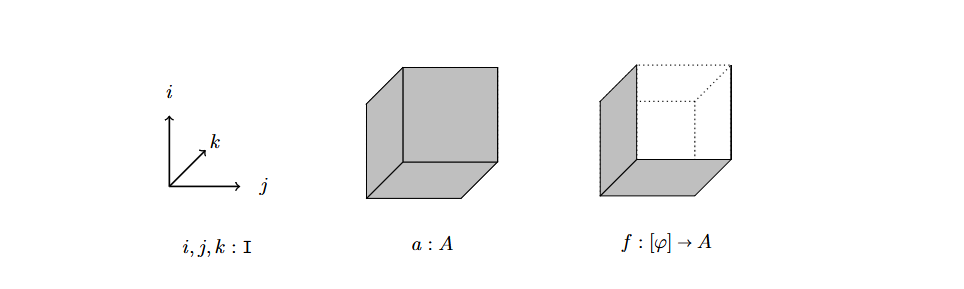
\includegraphics[width=0.9\textwidth]{partial}
\end{figure}
\end{example}

\begin{definition}[相容部分元的并]
称两个部分元 $f : [\varphi] \to A$ 和 $g : [\psi] \to A$ 是相容的，如果它们在都有定义的地方一致：
\begin{equation}
(\varphi, f) \smallsmile (\psi, g) \triangleq \forall(u : [\varphi])(v : [\psi]).\ f\,u = g\,v
\end{equation}
在这种情况下，我们可以形成它们的并 $f \cup g : [\varphi \lor \psi] \to A$，使得：
\[
\forall(u : [\varphi]).\ (f \cup g)\,u = f\,u \qquad \forall(v : [\psi]).\ (f \cup g)\,v = g\,v
\]
\end{definition}
要理解为什么，考虑拓扑斯中的以下推出方块：
\begin{figure}[htbp]
\centering

\includegraphics[width=0.9\textwidth]{partial_join}
\end{figure}
外层方块交换是因为 $(\varphi, f) \smallsmile (\psi, g)$ 成立，然后 $f \cup g$ 是推出诱导的唯一态射。注意，图1中的公理 $\ax{6}$ 意味着余纤维部分元素的集合在取兼容部分元素的二元并下封闭。

下面的引理给出了公理 $\ax{7}$ 和 $\ax{8}$ 的另一种刻画。由于我们上面注意到 $\mathtt{cof}\, \top$ 成立，引理的第(i)部分告诉我们，余纤维化在综合域论的意义上构成一个 \textit{dominance} [Ros86]；我们仅使用 $\mathtt{Cof}$ 的这一性质来从命题相等类型构造定义相等类型（见第5.3节）。

\begin{lemma}
\begin{enumerate}[label=(\roman*)]
\item 公理 $\ax{7}$ 等价于要求余纤维化类在复合下封闭。
\item 公理 $\ax{8}$ 等价于要求余纤维化类在 $\ttI$ 的指数化下封闭。
\end{enumerate}
\end{lemma}
\begin{proof}对于第(i)部分，首先假设 $\ax{7}$ 成立，且 $f : A \rightarrowtail B$ 和 $g : B \rightarrowtail C$ 是余纤维化。因此 $\forall(b : B). \mathtt{cof}(\exists(a : A). f\, a = b)$ 和 $\forall(c : C). \mathtt{cof}(\exists(b : B). g\, b = c)$ 都成立，我们希望证明 $\forall(c : C). \mathtt{cof}(\exists(a : A). g(f\, a) = c)$。注意到对于 $b : B$ 和 $c : C$

\[g b = c \implies (\exists(a : A). g(f a) = c) = (\exists(a : A). f a = b) \quad \text{由于 } g \text{ 是单态射}\]
\[\implies \mathtt{cof}(\exists(a : A). g(f a) = c) = \mathtt{cof}(\exists(a : A). f a = b) = \top\]
所以对于 $\varphi \triangleq \exists(b : B). g b = c$ 和 $\psi \triangleq \exists(a : A). g(f a) = c$，我们有 $\mathtt{cof} \, \varphi$ 和 $\mathtt{cof} \, \psi$。因此由 $\ax{7}$ 我们得到 $\mathtt{cof}(\phi \wedge \psi)$，它等于 $\mathtt{cof}(\psi)$，因为 $\psi \Rightarrow \varphi$。所以确实有 $\forall(c : C). \mathtt{cof}(\exists(a : A). g(f a) = c)$。

反之，假设余纤维化在复合下封闭，且 $\varphi, \psi : \Omega$ 满足 $\mathtt{cof} \, \varphi$ 和 $\mathtt{cof} \, \psi$。$\mathtt{cof} \, \varphi$ 成立等价于单态射 $[\varphi] \rightarrowtail 1$ 是余纤维化；并且由于

\[\varphi \implies (\psi = \varphi \wedge \psi) \implies (\mathtt{cof} \, \psi = \mathtt{cof}(\varphi \wedge \psi))\]

从 $\varphi \Rightarrow \mathtt{cof} \, \psi$ 我们得到 $\varphi \Rightarrow \mathtt{cof}(\varphi \wedge \psi)$，因此单态射 $[\varphi \wedge \psi] \rightarrowtail [\varphi]$ 是余纤维化。复合这些单态射，我们得到 $[\varphi \wedge \psi] \to 1$ 是余纤维化，即 $\mathtt{cof}(\varphi \wedge \psi)$ 成立。

对于第(ii)部分，首先假设 $\ax{8}$ 成立，且 $f : A \to B$ 是余纤维化。我们必须证明 $\ttI \to f : (\ttI \to A) \to (\ttI \to B)$ 也是余纤维化。给定 $\beta : \ttI \to B$，我们有

\[(\forall i : \ttI)(\exists a : A). f a = \beta i\]
\[\implies (\forall i : \ttI)(\exists! a : A). f a = \beta i \quad \text{(由于 } f \text{ 是单态射)}\]
\[\implies (\exists \alpha : \ttI \to A)(\forall i : \ttI). f(\alpha i) = \beta i \quad \text{(由拓扑斯中的唯一选择)}\]
\[\implies (\forall i : \ttI)(\exists a : A). f a = \beta i\]

因此 $(\forall i : \ttI)(\exists a : A). f a = \beta i$ 等于 $(\exists \alpha : \ttI \to A)(\forall i : \ttI). f(\alpha i) = \beta i$；而后者由拓扑斯中的函数外延性等于 $(\exists \alpha : \ttI \to A). (\ttI \to f)\alpha = \beta$。由于 $f$ 是余纤维化，对每个 $i : \ttI$ 我们有 $\mathtt{cof}(\exists(a : A)). f a = \beta i)$。因此由公理 $\ax{8}$，我们也有 $\mathtt{cof}((\forall i : \ttI)(\exists a : A). f a = \beta i)$，即 $\mathtt{cof}(\exists\alpha : \ttI \to A). (\ttI \to f)\alpha = \beta)$，正如 $\ttI \to f$ 成为余纤维化所需的那样。

反之，假设余纤维化在 $\ttI \to (\_)$ 下封闭，且 $\varphi : \ttI \to \Omega$ 满足 $(\forall i : \ttI). \mathtt{cof}(\varphi i)$。后者意味着 $\{i : \ttI \mid \varphi i\} \to \ttI$ 是余纤维化。因此单态射 $(\ttI \to \{i : \ttI \mid \varphi i\}) \to (\ttI \to \ttI)$ 也是余纤维化。由于 $id : \ttI \to \ttI$ 在该单态射的像中当且仅当 $(\forall i : \ttI). \varphi i$ 成立，我们得到 $\mathtt{cof}((\forall i : \ttI). \varphi i)$，正如公理 $\ax{8}$ 所要求的。
\end{proof}

\subsection{复合与填充结构}

图1中的公理 $\ax{5}-\ax{7}$ 给出了余纤维命题的简单性质，我们使用这些性质来定义纤维化的内部概念，推广 [CCHM18, 定义13]，并证明该概念在 $\Sigma$-、$\Pi$- 和 $\mathtt{Id}$-类型以及基本数据类型下封闭。

给定一个由区间索引的类型族 $A : {\ttI} \to \mathcal{U}$，我们将依赖函数类型 $\Pi_{\ttI} A \triangleq (i : {\ttI}) \to A\, i$ 的元素视为依赖类型的路径。我们称类型 $\square(\Pi_{\ttI} A)$ 的元素为\textit{余纤维部分路径}。给定 $(\varphi, f) : \square(\Pi_{\ttI} A)$，我们可以在区间的一个点 $i : {\ttI}$ 处求值，得到一个余纤维部分元素 $(\varphi, f) \,@\, i : \square(A\, i)$：

\begin{equation}(\varphi, f) \,@\, i \triangleq (\varphi, \lambda(u : [\varphi]) \to f\, u\, i) \end{equation}
对于 $A : {\ttI} \to \mathcal{U}$，一个\textit{从 $0$ 出发的填充}运算接受任意 $(\varphi, f) : \square(\Pi_{\ttI} A)$ 和任意满足 $(\varphi, f) \,@\, 0 \nearrow a_0$ 的 $a_0 : A\, 0$，并将 $(\varphi, f)$ 扩展为一个依赖路径 $g : \Pi_{\ttI} A$ 使得 $g\, 0 = a_0$。这是一种统一的\textit{同伦扩展与提升性质} (HELP) [May99, 第10章第3节]，它用余纤维命题在内部表述，而不是用余纤维化在外部表述。与 Cohen 等人相比，我们内部方法的一个特点是：当运算用余纤维命题的内部收集 $\mathtt{Cof}$ 表述时，他们对复合/填充运算的\textit{均匀性条件} [CCHM18, 定义13]（该条件使得人们能够避免经典 Kan 填充概念的非构造性方面 [BC15]）就变得自动满足了。

\begin{example}
  为了直观理解为什么这样的运算被称为填充，考虑下面的例子。为简单起见，假设 $A : {\ttI} \to \mathcal{U}$ 是常值族 $A \triangleq \lambda(\ul : {\ttI}) \to A'$。回顾我们将类型 ${\ttI}$ 的变量视为空间中的维度；因此，在环境上下文 $j, k : {\ttI}$ 中给定一个元素 $a : A$，我们将 $a$ 视为空间 $A$ 中的一个正方形。我们感兴趣的是将这个二维正方形扩展为一个三维立方体，如下所示。
\begin{figure}[htbp]
\centering
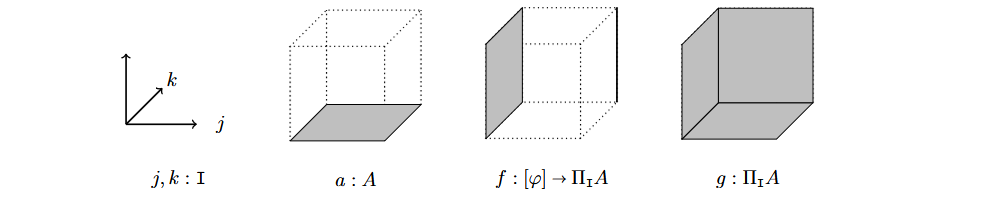
\includegraphics[width=0.9\textwidth]{comp}
\end{figure}

然而，假设我们已经知道如何在立方体的某些面和边上扩展 $a$，例如，在由 $\varphi \triangleq (j = 0) \lor (j = 1 \land k = 1)$ 指定的面/边上。这意味着我们有一个余纤维部分路径 $f : [\varphi] \to \Pi_{\ttI} A$，它在两者都有定义的地方与 $a$ 一致，即 $(\varphi, f) \,@\, 0 \nearrow a$。注意 $f$ 是部分路径而不是部分元素，因为在它定义的面/边上，它必须在扩展 $a$ 所沿的新维度的所有点上有定义，即 $\varphi$ 不能依赖于这个新维度。该数据的一个填充是一个立方体 $g : \Pi_{\ttI} A$，它与我们开始的面/边一致。也就是说，它扩展了 $f$ 并且在立方体的底面上与 $a$ 一致：$(\varphi, f) \nearrow g$ 且 $g\, 0 = a$。
\end{example}
由于我们没有假设区间上有任何用于反转路径的结构（见注记 3.2），我们还需要考虑从 1 出发的填充的对称概念。令

\begin{equation}\{0, 1\} \triangleq \{i : {\ttI} \mid i = 0 \lor i = 1\} \end{equation}
注意，由于公理 $\ax{2}$，这与布尔对象 $1 + 1$ 同构，因此存在一个函数
\begin{equation}\overline{\phantom{0}} : \{0, 1\} \to \{0, 1\} \end{equation}
满足 $\overline{0} = 1$ 和 $\overline{1} = 0$。在下面的内容中，我们不使用路径反转，而是用 $e : \{0, 1\}$ 参数化定义，并使用 (5.7) 来互换 $0$ 和 $1$。

\begin{definition}[填充结构]
  给定 $e : \{0, 1\}$，对于一个 ${\ttI}$-索引的类型族 $A : {\ttI} \to \mathcal{U}$，\textit{填充结构}的类型 $\mathtt{Fill} \ e \ A : \mathcal{U}$ 定义为：
\begin{align}
\mathtt{Fill}\,e\,A \triangleq &(\varphi : \Cof)(f : [\varphi] \to \Pi_\mathtt{I} A)(a : \{a' : A\,e \mid (\varphi, f) \ \,@\,\  e \nearrow a'\}) \to \\
&\{g : \Pi_\mathtt{I} A \mid (\varphi, f) \nearrow g \land g\,e = a\}\notag
\end{align}
\end{definition}
与先前的工作 [BCH14] 相比，[CCHM18] 的一个显著特征是，这种填充结构可以从更简单的\textit{复合}结构构造出来，该复合结构仅从一个端点的扩展产生另一端点的扩展。我们将使用公理 $\ax{3}-\ax{6}$ 从下面这个本文的主要概念中推导出这一点。

\begin{definition}[CCHM 纤维化]
类型 $\Gamma : \mathcal{U}$ 上的 \textit{CCHM 纤维化} $(A, \alpha)$ 是一个配备纤维化结构 $\alpha : \mathtt{isFib}\,A$ 的族 $A : \Gamma \to \mathcal{U}$，其中 $\mathtt{isFib} : \{\Gamma : \mathcal{U}\}(A : \Gamma \to \mathcal{U}) \to \mathcal{U}$ 定义为：
\begin{equation}
\mathtt{isFib}\,\{\Gamma\}\,A \triangleq (e : \{0, 1\})(p : \mathtt{I} \to \Gamma) \to \mathtt{Comp}\,e\,(A \circ p)
\end{equation}
这里 $\mathtt{Comp} : (e : \{0, 1\})(A : \mathtt{I} \to \mathcal{U}) \to \mathcal{U}$ 是 $\mathtt{I}$-索引族的\textit{复合结构}类型：
\begin{align}
\mathtt{Comp}\,e\,A \triangleq &(\varphi : \Cof)(f : [\varphi] \to \Pi_\mathtt{I} A) \to \\
&\{a_0 : A\,e \mid (\varphi, f) \ \,@\,\  e \nearrow a_0\} \to \{a_1 : A\,\overline{e} \mid (\varphi, f) \ \,@\,\  \overline{e} \nearrow a_1\}\notag
\end{align}
\end{definition}
展开定义，如果 $\alpha : \mathtt{isFib} \, A$，那么 $\alpha \ 0$ 满足：对于每条路径 $p : \ttI \to \Gamma$ 上的每个余纤维部分路径 $f : [\varphi] \to \Pi_{\ttI}(A \circ p)$，如果 $a_0 : A\ 0$ 扩展了部分元素 $(\varphi, f) \,@\, 0$，即 $\forall (u : [\varphi]) . f\ u\ 0 = a_0$，那么 $\alpha \ 0\ p\ \varphi\, f \ a_0 : A\ 1$ 扩展了 $(\varphi, f) \,@\, 1$，即 $\forall (u : [\varphi]) . f\ u\ 1 = \alpha \ 0 \ p \ \varphi \, f \ a_0$；对于 $\alpha \ 1$ 也有类似的性质。

\begin{definition}[CCHM 纤维化的 CwF]
  令 $\mathtt{Fib} \, \Gamma$ 为对象 $\Gamma$ 上的 CCHM 纤维化的类型，定义为：
\begin{equation}
  \mathtt{Fib} \, \Gamma \triangleq (A : \Gamma \to \mathcal{U}) \times \mathtt{isFib} \, A \end{equation}
\end{definition}
CCHM 纤维化在重索引下封闭：给定 $\gamma : \Delta \to \Gamma$ 和 $A : \Gamma \to \mathcal{U}$，我们得到一个函数 $\ul[\gamma] : \mathtt{isFib} \, A \to \mathtt{isFib}(A \circ \gamma)$，定义为 $\alpha[\gamma] \ e \ p \triangleq \alpha \ e \ (\gamma \circ p)$。因此我们得到一个函数 $\ul[\ul] : (\Delta \to \Gamma) \to \mathtt{Fib} \, \Gamma \to \mathtt{Fib} \, \Delta$，由下式给出：
\begin{equation}(A, \alpha)[\gamma] \triangleq (A \circ \gamma, \alpha[\gamma])\end{equation}
它是函子性的：$(A, \alpha)[id] = (A, \alpha)$ 且 $(A, \alpha)[g \circ f] = (A, \alpha)[g][f]$。由此可知，通过将族取为每个 $\Gamma : \mathcal{U}$ 上的 CCHM 纤维化 $(A, \alpha) : \mathtt{Fib} \, \Gamma$，并将这种族的元素取为依赖函数 $(x : \Gamma) \to A\ x$，$\mathtt{Fib}$ 具有 CwF 的结构。

\begin{remark}[纤维化对象]
  如果常值族 $\lambda(\ul : 1) \to A$ 在终对象 $1$ 上具有一个纤维化结构，则称 $A : \mathcal{U}$ 为\textit{纤维化对象}。注意，如果 $(A, \alpha) : \mathtt{Fib} \, \Gamma$ 是一个纤维化，那么对于每个 $x : \Gamma$，类型 $A\ x : \mathcal{U}$ 是纤维化的，其纤维化结构由通过映射 $\lambda(\ul : 1) \to x : 1 \to \Gamma$ 重索引 $\alpha$ 给出。然而反过来不成立：拥有一个纤维化结构的族，即 $(x : \Gamma) \to \mathtt{isFib}(\lambda(\ul : 1) \to A\ x)$ 的一个元素，比拥有 $A : \Gamma \to \mathcal{U}$ 的一个纤维化结构要弱。要理解原因，考虑由下式定义的族 $P : {\ttI} \to \mathcal{U}$
\begin{equation}P\ i \triangleq [i = 0]\end{equation}
对于每个 $i : {\ttI}$，纤维 $P\ i : \mathcal{U}$ 是一个纤维化对象，具有一个纤维化结构 $\rho_i : \mathtt{isFib}(\lambda(\ul : 1) \to P\ i)$，由 $\rho_i \ e \ p \ \phi \ f \ x \triangleq x$ 给出。然而，不可能构造一个 $\rho : \mathtt{isFib} \, P$。因为如果存在，那么我们可以定义 $\rho \ 0 \ id \ \bot \, \mathtt{elim}_\emptyset \ * : [1 = 0]$；与 $\ax{2}$ 结合将导致矛盾。
\end{remark}

如果 $\alpha : \mathtt{Fill} \, e \, A$，那么 $\lambda \varphi \, f \, a \to \alpha \ \varphi \ f \ a \ \bar{e} : \mathtt{Comp} \ e \, A$，因此每个填充结构都产生一个复合结构。反过来，CCHM 纤维化的复合结构产生填充结构：

\begin{lemma}[从复合结构构造填充结构]
给定 $\Gamma : \mathcal{U}$，$A : \Gamma \to \mathcal{U}$，$e : \{0, 1\}$，$\alpha : \mathtt{isFib}\ A$ 和 $p : \mathtt{I} \to \Gamma$，存在一个填充结构 $\mathtt{fill}\ e\ \alpha\ p : \mathtt{Fill}\ e\ (A \circ p)$，它在 $\overline{e}$ 处与 $\alpha$ 一致，即：
\begin{align}
\forall(\varphi : \Cof)(f : [\varphi] \to \Pi_\mathtt{I} A)(a : A(p&\ e)).\notag\\
&(\varphi, f) \ @\  e \nearrow a \Rightarrow \mathtt{fill}\ e\ \alpha\ p\ \varphi\ f\ a\ \overline{e} = \alpha\ e\ p\ \varphi\ f\ a
\end{align}
此外，$\mathtt{fill}$ 在重索引下是\textit{稳定的}，在这个意义上，对于所有 $\gamma : \Delta \to \Gamma$ 和 $p : \mathtt{I} \to \Delta$：
\begin{equation}
\mathtt{fill}\ e\ \alpha\ (\gamma \circ p) = \mathtt{fill}\ e\ (\alpha[\gamma])\ p
\end{equation}
\end{lemma}
\begin{proof}
  从复合构造填充的过程遵循 [CCHM18, 第4.4节]，但仅使用 $\Gamma$ 上的 connection 代数结构（公理 $\ax{3}$ 和 $\ax{4}$），而不是 de Morgan 代数结构。假设 $\Gamma : \mathcal{U}, A : \Gamma \to \mathcal{U}, e : \{0,1\}, \alpha : \mathtt{isFib} \, A, p : \Gamma \to \Gamma, \varphi : \mathtt{Cof}, f : [\varphi] \to \Pi_{\ttI} (A \circ p), a : A(p(e))$ 满足 $(\varphi, f) \,@\, e \sim a$，以及 $i : {\ttI}$。然后使用定义 5.3，我们可以定义

\[\mathtt{fill} \, e \, \alpha \, p \, \varphi \, f \, a \, i \triangleq \alpha \, e \, (p' \, i) \, (\varphi \lor i = e) \, (f' \, i \cup g \, i) \, a \tag{5.16}\]

其中

- $p' : {\ttI} \to \Gamma \to \Gamma$ 定义为 $p' \, i \, j \triangleq p(i \sqcap e \, j)$
- $f' : (i : {\ttI}) \to [\varphi] \to \Pi_{\ttI} (A \circ (p' \, i))$ 定义为 $f' \, i \, u \, j \triangleq f \, u \, (i \sqcap e \, j)$
- $g : (i : {\ttI}) \to \{g' : [i = e] \to \Pi_{\ttI} (A \circ (p' \, i)) \mid (\varphi, f' \, i) \sim (i = e, g')\}$ 定义为 $g \, i \, v \, j \triangleq a$

这里 $\Gamma_e$ 由 $\Gamma_0 \triangleq \Gamma$ 和 $\Gamma_1 \triangleq \bot$ 给出。最后，性质 (5.15) 直接从定义 (5.12) 和 (5.16) 得到。□
\end{proof}
与 [BCH14] 相比，填充可以从复合定义这一事实大大简化了通过通常的类型构造提升纤维化结构的过程，如下面两个定理所示。它们的证明是 [CCHM18, 第4.5节] 中证明的内化，只是我们避免了 Cohen 等人对 de Morgan 对合的使用。

\section{Glueing}

在本节中，我们给出 Cohen 等人 [CCHM18] 所提出的 \textit{glueing} 构造的内部表述。Glueing 类似于类型族的复合结构（定义 5.7），但它不是涉及类型的部分路径，而是涉及类型之间的部分等价。Glueing 对第 7 节中与 univalence [Uni13] 相关的构造至关重要。

我们首先定义余纤维部分类型（即函数 $ A : [\varphi] \to \mathcal{U} $，其中 $ \varphi : \mathtt{Cof} $）的 glueing 构造：

\begin{definition}[Glueing]
  给定 $ \varphi : \mathtt{Cof}, A : [\varphi] \to \mathcal{U}, B : \mathcal{U} $ 和 $ f : (u : [\varphi]) \to A\ u \to B $，类型 $ \mathtt{Glue}\ \varphi\ A\ B\ f : \mathcal{U} $ 定义为

\begin{equation} 
  \mathtt{Glue}\ \varphi\ A\ B\ f \triangleq (a : (u : [\varphi]) \to A\ u) \times \{b : B \mid \forall (u : [\varphi]). f\ u\ (a\ u) = b\}
\end{equation}
\end{definition}
该类型的元素由对 $ (a, b) $ 组成，其中 $ a $ 是部分类型 $ A $ 的部分元素，$ b $ 是类型 $ B $ 的元素，使得将 $ f $ 应用于 $ a $ 得到 $ B $ 的一个部分元素，该部分元素可扩展到 $ b $。当 $ \varphi = \top $ 时，$ A $ 和 $ f $ 都是整体的，因此 $ \mathtt{Glue}\ \varphi\ A\ B\ f $ 本质上由每个 $ a : A $ 对应的对 $ (a, f\ a) $ 组成，从而显然与 $ A $ 同构。当 $ \varphi = \bot $ 时，$ A $ 和 $ f $ 都被唯一确定，并且 $ \mathtt{Glue}\ \varphi\ A\ B\ f $ 由每个 $ b : B $ 对应的对 $ (\mathtt{elem}_{\emptyset}, b) $ 组成，从而显然与 $ B $ 同构。

我们现在将这一 glueing 运算从余纤维部分类型扩展到\textit{余纤维部分类型族}：

\begin{definition}[余纤维部分族]
  给定一个对象 $ \Gamma : \mathcal{U} $ 和一个余纤维性质 $ \Phi : \Gamma \to \mathtt{Cof} $，定义\textit{$ \Gamma $ 被 $ \Phi $ 的限制}为
\begin{equation}
\Gamma | \Phi \triangleq (x : \Gamma) \times [\Phi\ x]
\end{equation}
\end{definition}
因此 $ \Gamma | \Phi : \mathcal{U} $ 且存在由第一投影给出的单态射 $ \iota : \Gamma | \Phi \rightarrowtail \Gamma $。（注意 $ \Gamma | \Phi $ 同构于 comprehension 子类型 $ \{x : \Gamma \mid \Phi\ x\} $，但我们使用上述表示以使 $ \Phi\ x $ 的证明在各种构造中更加明确。）然后，给定对象 $ \Gamma : \mathcal{U} $ 和一个余纤维性质 $ \Phi : \Gamma \to \mathtt{Cof} $，一个\textit{余纤维部分类型族}是限制 $ \Gamma | \Phi $ 上的一个类型族 $ A $，即 $ A : (\Gamma | \Phi) \to \mathcal{U} $。

\begin{definition}[族的 Glueing]
  我们将 glueing 运算从类型提升到类型族如下。给定 $ \Gamma : \mathcal{U}, \Phi : \Gamma \to \mathtt{Cof}, A : \Gamma |\Phi \to \mathcal{U}, B : \Gamma \to \mathcal{U} $ 和 $ f : (x : \Gamma)(v : [\Phi\ x]) \to A(x, v) \to B\,x $，定义族 $ \mathtt{Glue} \, \Phi \, A \, B \, f : \Gamma \to \mathcal{U} $ 为
\begin{equation} \mathtt{Glue} \, \Phi \, A \, B \, f \, x \triangleq \mathtt{Glue}(\Phi \, x)(A(x, \ul))(B \, x)(f(x, \ul)) \end{equation}
\end{definition}
Glueing 构造对任意映射 $ f : (x : \Gamma)(v : [\Phi\ x]) \to A(x, v) \to B\ x $ 都有效。然而，我们希望看到这一构造能够提升到 CCHM 纤维化的 CwF 上。这意味着当 $ A $ 和 $ B $ 都具有纤维化结构时，Glue $ \Phi A\,Bf $ 也应具有纤维化结构，这会对 $ f $ 提出一些要求。我们首先引入\textit{扩展结构}的概念：

\begin{definition}[扩展结构]
  扩展结构的类型 $ \mathtt{Ext} : \mathcal{U} \to \mathcal{U} $ 定义为
\[ \mathtt{Ext}\,A \triangleq (\tilde{a} : \square A) \to \{a : A \mid \tilde{a} \nearrow a\} \]
\end{definition}
为类型 $ A : \mathcal{U} $ 拥有一个扩展结构，使我们能够将 $ A $ 的任何部分元素扩展为一个整体元素。我们称一个族 $ A : \Gamma \to \mathcal{U} $ 拥有扩展结构，如果它的每个纤维都有，并滥用记号写作

\[ \mathtt{Ext}\,A \triangleq (x : \Gamma) \to \mathtt{Ext}(A\ x) \]

族 $ A : \Gamma \to \mathcal{U} $ 的扩展结构类似于拥有一个复合结构，因为两者都允许我们扩展部分元素；事实上，每个具有扩展结构的族都是纤维化。然而，扩展结构不需要从中扩展/复合的整体元素，因此它实际上是比复合结构更强的概念。首先注意，为 $ A : \mathcal{U} $ 拥有扩展结构意味着 $ A $ 是 inhabited，因为我们总是可以扩展空的部分元素。此外，给定任意元素 $ a : A $，我们可以使用扩展结构证明它与空部分元素的扩展是路径相等的。综合这些事实可知 $ A $ 是 *可收缩的*：

\begin{definition}[可收缩性 [Uni13, 第3.11节]]
  一个类型 $ A $ 被称为 *可收缩的*，如果它有一个收缩中心 $ a_0 : A $ 且每个元素 $ a : A $ 都命题等于 $ a_0 $，即存在一条路径 $ a_0 \sim a $。因此，类型是可收缩的当且仅当 $ \mathtt{Contr}\,A $ 是 inhabited，其中 $ \mathtt{Contr} : \mathcal{U} \to \mathcal{U} $ 定义为
\[ \mathtt{Contr}\,A \triangleq (a_0 : A) \times ((a : A) \to a_0 \sim a) \]
与扩展结构类似，我们称族 $ A : \Gamma \to \mathcal{U} $ 是可收缩的，如果它的每个纤维都是，并写作
\[ \mathtt{Contr}\,A \triangleq (x : \Gamma) \to \mathtt{Contr}(A\ x) \]
\end{definition}
如上所述，族 $ A : \Gamma \to \mathcal{U} $ 拥有扩展结构蕴含 $ A $ 既是纤维化的又是可收缩的。事实上，反过来也成立（[CCHM18, 引理5]）：

\begin{lemma}
存在函数
\begin{align}
&\mathtt{fromExt} : \{\Gamma : \mathcal{U}\}\{A : \Gamma \to \mathcal{U}\} \to \mathtt{Ext}\ A \to \mathtt{isFib}\ A \times \mathtt{Contr}\ A \\
&\mathtt{toExt} : \{\Gamma : \mathcal{U}\}\{A : \Gamma \to \mathcal{U}\} \to \mathtt{isFib}\ A \to \mathtt{Contr}\ A \to \mathtt{Ext}\ A
\end{align}
\end{lemma}

\begin{proof}
  给定 $ \Gamma : \mathcal{U}, A : \Gamma \to \mathcal{U} $ 和 $ \varepsilon : \mathtt{Ext}\,A $，我们定义 $ \alpha : \text{isFib } A $

\[ \alpha e p \varphi f a_0 \triangleq \varepsilon (p \bar{e}) ((\varphi, f) @ \bar{e}) \]

对于每个 $ x : \Gamma $，我们使用完全未定义的余纤维部分元素 $ (\perp, \text{elim}_\theta) : \square A $ 来定义 $ a_0 : A $

\[ a_0 \triangleq \varepsilon x (\perp, \text{elim}_\theta) \]

对于每个 $ a : A x $ 和 $ i : I $，我们有 $ \lambda_- \to a : [i = 1] \to A x $；因此我们得到一条路径 $ p_a : I \to A x $

\[ p_a i \triangleq \varepsilon x (i = 1, \lambda_- \to a) \]

根据 Ext $ A $ 的定义，有 $ p_a 1 = \varepsilon x(\top, \lambda \to a) = a $，并且由 $ \ax{2} $ 有 $ p_a 0 = \varepsilon x(\bot, \text{elim}_\theta) = a_0 $。因此 $ p_a : a_0 \sim a $。因此 $ A x $ 是可收缩的。综上所述，给定 $ \varepsilon : \mathtt{Ext}\,A $，我们可以定义类型为 isFib $ A $ 和 Contr $ A $ 的元素。因此存在函数 fromExt : $\{\Gamma : \mathcal{U}\} \{A : \Gamma \to \mathcal{U}\} \to \mathtt{Ext}\,A \to \text{isFib } A \times \mathtt{Contr}\,A$。

反之，给定 $ \Gamma : \mathcal{U}, A : \Gamma \to \mathcal{U}, \alpha : \text{isFib } A, \langle a_0, p \rangle : \mathtt{Contr}\,A $，注意对于任意 $ x : \Gamma, \varphi : \mathtt{Cof}, f : [\varphi] \to A x $，有 $ (p x) \circ f : [\varphi] \to (I \to A x) $ 使得 $ \forall (u : [\varphi]). ((p x) \circ f) u : a_0 x \sim f u $；因此 $ (\varphi, (p x) \circ f) @ 0 \nearrow (a_0 x) $，从而定义

\[ \varepsilon x (\varphi, f) \triangleq \alpha 0 (\lambda \to x) \varphi ((p x) \circ f) (a_0 x) \]

我们得到 $ \varepsilon x (\varphi, f) : A x $。此外，由于 $ (\varphi, (p x) \circ f) @ 1 = (\varphi, f) $，由 $ \alpha $ 的类型可得 $ (\varphi, f) \nearrow \varepsilon x (\varphi, f) $。因此 $ \varepsilon x (\varphi, f) : \mathtt{Ext}(A x) $，如所需。
\end{proof}

现在我们来到本节的主要结果：证明纤维化在 glueing 下封闭。证明这一点要求函数 $ f $ 是一个等价：

\begin{definition}[等价 [Uni13, 第4.4节]]
给定类型 $A, B : \mathcal{U}$，函数 $f : A \to B$ 是一个\textbf{等价}，如果类型 $\mathtt{Equiv}\ f$ 是非空的，其中
\[
\mathtt{Equiv}\ f \triangleq (b : B) \to \mathtt{Contr}((a : A) \times f\ a \sim b)
\]
\end{definition}
同样，这显然可以提升到族：给定 $\Gamma : \mathcal{U}$，$A, B : \Gamma \to \mathcal{U}$ 和 $f : (x : \Gamma) \to A\ x \to B\ x$，定义
\[
\mathtt{Equiv}\ f \triangleq (x : \Gamma) \to \mathtt{Equiv}(f\ x)
\]
\begin{theorem}[Glueing 的复合]
令 $\Phi, A, B$ 和 $f$ 如定义 5.4.2 中所述。那么如果 $A$ 和 $B$ 都有纤维化结构且 $f$ 具有等价的结构，则 $\mathtt{Glue}\ \Phi\,A\,B\,f$ 具有纤维化结构。换言之，存在一个函数
\begin{align}
\mathtt{isFib}_{\mathtt{Glue}} : &\{\Gamma : \mathcal{U}\}\{\Phi : \Gamma \to \mathtt{Cof}\}\{A : \Gamma|\Phi \to \mathcal{U}\}\{B : \Gamma \to \mathcal{U}\} \\
&(f : (x : \Gamma)(u : [\Phi\ x]) \to A(x, u) \to B\ x) \to\notag\\
&((x : \Gamma)(v : [\Phi\ x]) \to \mathtt{Equiv}(f\ x\ v)) \to\notag\\
&\mathtt{isFib}\ A \to \mathtt{isFib}\ B \to \mathtt{isFib}(\mathtt{Glue}\ \Phi\,A\,B\,f)\notag
\end{align}
\end{theorem}
\begin{proof}
  给定 $ \Gamma : \mathcal{U}, \Phi : \Gamma \to \mathtt{Cof}, A : \Gamma | \Phi \to \mathcal{U}, B : \Gamma \to \mathcal{U}, f : (x : \Gamma)(u : [\Phi\ x]) \to A(x, u) \to B\,x, eq : (x : \Gamma)(u : [\Phi\ x]) \to \mathtt{Equiv}(f x u), \alpha : \mathtt{isFib} A, \beta : \mathtt{isFib} B $，我们希望定义类型为 $ \mathtt{isFib}(\mathtt{Glue} \Phi A\,B f) $ 的元素。因此，取

\[ e : \{0, 1\}, p : \Gamma \to \Gamma, \psi : \mathtt{Cof}, q : [\psi] \to \Pi_I(\mathtt{Glue} \Phi A\,B f) \]
\[ (a_0, b_0) : \{(a_0, b_0) : (\mathtt{Glue} \Phi A\,B f)(p e) \mid (\psi, q) @ e \nearrow (a_0, b_0)\} \]

我们的目标是定义 $ (a_1, b_1) : (\mathtt{Glue} \Phi A\,B f) x $ 使得 $ (\psi, \tilde{a}_1) \nearrow a_1 $ 和 $ (\psi, \tilde{b}_1) \nearrow b_1 $，其中 $ x : \Gamma, \tilde{a}_1 : [\psi] \to ((u : [\Phi\ x]) \to A(x, u)) $ 和 $ \tilde{b}_1 : [\psi] \to B\,x $ 定义为

\[ x \triangleq p \bar{e} \]
\[ \tilde{a}_1 v \triangleq \text{fst}(q v \bar{e}) \]
\[ \tilde{b}_1 v \triangleq \text{snd}(q v \bar{e}) \]

并且由 Glue $ \Phi A\,B f $ 的定义满足 $ \forall (v : [\psi])(u : [\Phi\ x]). f x u (\tilde{a}_1 v u) = \tilde{b}_1 v $。

我们首先在 $ B $ 中沿 $ p $ 复合以得到 $ b'_1 : B\,x $，它可以看作是 $ b_1 $ 的第一个近似：

\[ b'_1 \triangleq \beta e p \psi (\lambda(v : [\psi])(i : I) \to \text{snd}(q v i)) b_0 \]

回忆 $ a_1 $ 的类型是 $ (u : [\Phi\ x]) \to A(x, u) $，因此我们假设 $ u : [\Phi\ x] $ 以定义类型 $ A(x, u) $ 的一个元素。注意我们不能简单地在 $ A $ 中沿 $ p $ 复合，因为我们不知道对所有 $ i : I $ 有 $ \Phi(p i) $ 成立。相反，我们将使用等价结构来定义 $ a_1 $。

令 $ C \triangleq (a : A(x, u)) \times f x u a \sim b'_1 $ 为 $ f x u $ 在 $ b'_1 $ 处的纤维。使用定理 5.11 和 5.15，以及 $ A $ 和 $ B $ 都是纤维化（分别由 $ \alpha $ 和 $ \beta $ 见证）的事实，我们可以推出 $ C $ 是一个纤薄对象。结合 $ eq x u b'_1 : \mathtt{Contr} C $ 的事实，我们可以使用引理 6.6 定义 $ \varepsilon : \mathtt{Ext} C $。然后我们可以定义

\[ (\psi, (\lambda(v : [\psi]) \to \tilde{a}_1 v u, \text{ refl } \circ \tilde{b}_1)) : \square C \]

这是良定义的，因为如上所述，有 $ \forall (v : [\psi]) . f x u (\tilde{a}_1 v u) = \tilde{b}_1 v $，并且由复合结构的类型，有 $ (\psi, \tilde{b}_1) \nearrow b'_1 $，从而给定 $ v : [\psi] $，有 $ \text{refl}(\tilde{b}_1 v) : f x u (\tilde{a}_1 v u) \sim b'_1 $。现在我们可以定义

\[ \varepsilon (\psi, (\lambda(v : [\psi]) \to \tilde{a}_1 v u, \text{ refl } \circ \tilde{b}_1)) : C \]

解除假设 $ u : [\Phi\ x] $ 并取上述定义的对的第一和第二个投影，我们得到：

\[ a_1 : (u : [\Phi\ x]) \to A(x, u) \quad pb : (u : [\Phi\ x]) \to f x u (a_1 u) \sim b'_1 \]

现在我们有了 $ a_1 $ 和 $ b'_1 $，使得 $ \tilde{a}_1 \nearrow a_1 $ 和 $ \tilde{b}_1 \nearrow b'_1 $。然而，我们不能直接取 $ b_1 $ 为 $ b'_1 $，因为我们不知道 $ \forall (u : \Phi\ x) . f x u (a_1 u) = b'_1 $，因此不能断定 $ (a_1, b'_1) : (\mathtt{Glue} \Phi A\,B f) x $。为解决这个问题，我们在 $ B\,x $ 中进行最后一次复合，以“修正” $ b'_1 $ 使其满足该性质。考虑以下并：

\[ pb \cup (\text{refl} \circ \tilde{b}_1) : [\Phi\ x \lor \psi] \to \Pi_I(Bx) \]

这是良定义的，因为 $ pb $ 是通过扩展 $ \text{refl} \circ \tilde{b}_1 $ 定义的，因此它们在两者都有定义的地方必然相等。我们利用它在 $ B\,x $ 中进行最后一次复合：

\[ b_1 \triangleq \beta 1 (\lambda(- : I) \to x) (\Phi\ x \lor \psi) (pb \cup (\text{refl} \circ \tilde{b}_1)) b'_1 \]

现在我们得到 $ (a_1, b_1) : (\mathtt{Glue} \Phi A\,B f) x $ 且满足 $ (\psi, \tilde{a}_1) \nearrow a_1 $ 和 $ (\psi, \tilde{b}_1) \nearrow b_1 $，如所需。
\end{proof}
现在我们获得了一种解释 [CCHM18] 中 glueing 运算的方法，该方法满足了一些必要条件；参见 [CCHM18, 图4]。然而，当前的构造未能满足：当沿着包含 $ \iota : \Gamma |\Phi \rightarrowtail \Gamma $ 重索引时，$ \mathtt{Glue}\ \Phi\ A\ B\ f $ 应等于 $ A $。实际上，这个等式应该在 CCHM 纤维化的 CwF 中成立。这意味着不仅应有 $ A = (\mathtt{Glue}\ \Phi\ A\ B\ f) \circ \iota : \Gamma |\Phi \to \mathcal{U} $，而且重索引定理 6.8 中导出的纤维化结构应得到我们开始时的同一个纤维化结构。精确地说，我们需要：
\begin{equation} (A, \alpha) = (\mathtt{Glue}\ \Phi\ A\ B\ f, \mathtt{isFib}_{\mathtt{Glue}} \, f \ eq \ \alpha \ \beta)[\iota] \end{equation}

目前我们所知的是，族 $ A $ 和 $ (\mathtt{Glue}\ \Phi\ A\ B\ f) \circ \iota $ 在以下意义上是同构的：

\begin{definition}[同构]
  给定对象 $ A, B : \mathcal{U} $，$ A $ 与 $ B $ 之间的同构是一个具有双边逆的函数 $ f : A \to B $。令 $ A \cong B $ 为 $ A $ 与 $ B $ 之间同构的类型，定义为
\[ A \cong B \triangleq \{f : A \to B \mid (\exists g : B \to A) (g \circ f = id) \land (f \circ g = id)\} \]
\end{definition}
如果存在一个同构 $ f : A \cong B $，则称 $ A $ 与 $ B $ 同构。这一概念以明显的逐点方式提升到族。同构具有内部类型论的外延相等意义下的逆，而等价则只有路径相等意义下的逆。

我们分两步得到 (6.7)。首先，我们使用公理 $ \ax{9} $ 来\textit{严格化} glueing 构造，得到一个新的严格形式的 glueing，记作 $\mathtt{SGlue}$，使得 $\mathtt{Glue}\ \Phi \, A\,B \, f \cong  \mathtt{SGlue}\ \Phi \, A\,B \, f $，但满足 $ A = (\mathtt{SGlue} \, \Phi \, A\,B \, f) \circ \iota $。然后我们使用公理 $ \ax{8} $ 来调整 $\mathtt{SGlue}$ 上的纤维化结构，使得沿 $ \iota $ 重索引后等于 $ A $ 上的纤维化结构。这些步骤的顺序似乎并不重要；我们同样可以先调整 $\mathtt{Glue}$ 上的纤维化结构，然后用这个新的纤维化结构来严格化 $\mathtt{Glue}$。

\begin{remark}
除了使用拓扑斯的内部语言之外，我们获得具有良好性质的 glueing 运算的方法与 Cohen 等人 [CCHM18] 所采取的方法不同，在那里 glueing 是直接定义的，并具有所有需要的性质。不过，我们仍然可以看到最终两个步骤在原始工作中的位置。严格化可见于 [CCHM18, 定义15] 中对 $ \varphi \rho = 1_{\mathbb{F}} $ 的情形拆分；更多细节见第 8.2 节。Cohen 等人没有先为 glueing 定义一个初始的复合结构然后修改它以获得所需的重索引性质，而是直接定义了复合结构。从 [CCHM18, 第6.2节] 中移除所有 $ \forall $ 算子的使用将得到我们的初始复合结构，然后我们在单独的步骤中使用 $\mathtt{Cof}$ 在 $ \forall(i : I) $ 下的封闭性（公理 $ \ax{8} $）来修改这个复合。我们更喜欢这种方法，因为它简化了 glueing 的核心复合结构，并更明确地揭示了 $ \ax{8} $ 在构建立方类型论模型中所起的作用。
\end{remark}
现在我们回忆图1中的公理 $ \ax{9} $：
\begin{align*}
\ax{9} : &\{\varphi : \mathtt{Cof}\}(A : [\varphi] \to \mathcal{U})(B : \mathcal{U})(s : (u : [\varphi]) \to (A\ u \cong B)) \to\\
&(B' : \mathcal{U}) \times \{s' : B' \cong B \mid \forall(u : [\varphi]).\ A\ u = B' \land s\ u = s'\}
\end{align*}
这表述了：任何在其定义处处处同构于一个整体类型 $ B $ 的部分类型 $ A $ 都可以扩展为一个整体类型 $ B' $，且 $ B' $ 同构于 $ B $。我们在第 8.2 节中研究为什么立方预层拓扑斯 [CCHM18] 满足这条公理。给定 $ \ax{8} $，定义严格形式的 glueing 是直接的。

**定义 6.11 (严格 Glueing).** 给定 $ \Phi, A, B, f $ 如定义 6.3，定义

\[ \mathtt{SGlue} \, \Phi \, A \, B \, f : \Gamma \to \mathcal{U} \]

如下：对 $ x : \Gamma $，设 $ \varphi \triangleq \Phi\ x $。由定义 6.1，我们有类型 $ \mathtt{Glue} \, \varphi \, (A(x,-)) \, (B\,x) \, (f x) $。由 $ \ax{9} $，存在一个类型 $ G x : \mathcal{U} $ 和一个同构 $ s_x : G x \cong B\,x $，使得 $ \forall (u : [\varphi]). A(x, u) = G x $ 且 $ f x u = s_x $。因此，我们只需定义 $ \mathtt{SGlue} \, \Phi \, A \, B \, f \, x \triangleq G x $。注意，由构造，有 $ (\mathtt{SGlue} \, \Phi \, A \, B \, f) \circ \iota = A $。

**定理 6.12 (严格 Glueing 的纤维化结构).** 在定理 6.8 的假设下，$\mathtt{SGlue}\ \Phi\ A\ B\ f $ 具有一个纤维化结构。

**证明.** 容易证明（逐纤维的）同构保持纤维化结构。因此，我们可以沿着 $ \ax{9} $ 给出的同构，将定理 6.8 中 $ \mathtt{isFibGlue} $ 得到的结构运输到 $\mathtt{SGlue}$ 上，从而得到 $\mathtt{SGlue}$ 的一个纤维化结构。

本节的最后一步是使用公理 $ \ax{9} $ 来调整 $\mathtt{SGlue}$ 的复合结构，以恢复 $ A $ 上的原始复合结构。

**定理 6.13 (调整复合结构).** 给定 $ \Gamma : \mathcal{U} $ 和 $ \Phi : \Gamma \to \mathtt{Cof} $，设 $ \iota : \Gamma | \Phi \to \Gamma $ 如定义 6.2。对于任意 $ G : \Gamma \to \mathcal{U} $，$ \alpha : \mathtt{isFib}(G \circ \iota) $ 和 $ \gamma : \mathtt{isFib} \, G $，存在一个复合结构 $ \gamma' : \mathtt{isFib} \, G $ 使得 $ \alpha = \gamma'[\iota] $。

**证明.** 给定如上所述的 $ \Gamma, \Phi, A, \alpha, \gamma $，使用公理 $ \ax{8} $（以及 $ \ax{6} $），我们可以如下定义 $ \gamma' $：

\[ \gamma' e p \psi f g \triangleq \gamma e p (\psi \lor (\forall(i : I). \Phi(p(i)))) (f \cup f') g \tag{6.10} \]

其中 $ f' : [\forall(i : I). \Phi(p(i))] \to \Pi_I G $ 定义为 $ f' u \triangleq \text{fill } e \alpha (\lambda i \to (p, u i)) \psi f g $。$ f $ 与 $ f' $ 的兼容性源于我们在定义 $ f' $ 时使用了 $ \psi $ 和 $ f $，因此由填充的性质，$ f' $ 在它们相互定义的地方必然与 $ f $ 一致。

**推论 6.14.** 给定 $ \Gamma : \mathcal{U}, \Phi : \Gamma \to \mathtt{Cof}, (A, \alpha) : \text{Fib}(\Gamma | \Phi), (B, \beta) : \text{Fib} \, \Gamma $ 和 $ f : (x : \Gamma)(v : [\Phi\ x]) \to A(x, v) \to B\,x $，存在 $ (G, \gamma) : \text{Fib} \, \Gamma $ 使得 $ (A, \alpha) = (G, \gamma)[\iota] $。

**证明.** 只需取 $ G = \mathtt{SGlue} \, \Phi \, A \, B \, f $；由定理 6.12 得到 $ G $ 的一个复合结构，然后使用定理 6.13 调整该复合结构，得到一个新的满足所需等式的复合结构 $ \gamma $。

\section{单值性}

Voevodsky 在 CwF（至少具有 $\Sigma$-、$\Pi$- 和 $\mathtt{Id}$-类型）中对宇宙 $\mathcal{V}$ 提出的\textit{单值公理} [Uni13, 第2.10节] 指出：对每个 $A, B : \mathcal{V}$，从 $\mathtt{Id}_\mathcal{V} A B$ 到 $(f : A \to B) \times \text{Equiv } f$ 的典范函数是一个等价。Cohen 等人在立方集的预层拓扑斯（所关联的 CwF）中构造了一个宇宙，其类型族对具有小纤维的 CCHM 纤维化（对于元理论中合适的小性概念）是通用的，并证明它满足单值公理。他们通过适配预层范畴上的 Hofmann-Streicher 宇宙构造 [HS99] 来实现这一点。仅使用一般拓扑斯的内部类型论无法表达他们的宇宙构造，原因我们在下面的注记 7.5 中讨论。在最近的工作中，作者与 Licata 和 Spitters [LOPS18] 一起展示了如何在内部类型论的模态扩展中公理化 CCHM 宇宙构造。这里我们仅证明单值性的一个版本，而不涉及纤维化宇宙的参考。

为了理解这可能意味着什么，考虑以下情况：如果存在一个宇宙 $\mathcal{V}$，其元素是 CCHM 纤维化的编码，那么给定由进入宇宙的函数 $a, b : \Gamma \to \mathcal{V}$ 命名的纤维化 $(A, \alpha), (B, \beta) : \text{Fib } \Gamma$，$a$ 与 $b$ 之间的路径等式（通过 Currying）给出一个函数 $p : \Gamma \times I \to \mathcal{V}$ 使得对所有 $x : \Gamma$ 有 $p(x, 0) = a x$ 和 $p(x, 1) = b x$。于是 $p$ 命名了一个纤维化 $(P, \rho) : \text{Fib}(\Gamma \times I)$，满足 $(P, \rho)[\langle id, 0 \rangle] = (A, \alpha)$ 和 $(P, \rho)[\langle id, 1 \rangle] = (B, \beta)$。后者给出了一种类型族之间的路径等式概念，无论是否存在这样的 $\mathcal{V}$，我们将在本节中研究它与纤维化之间的等价的关系。

为了更形式化地给出定义，我们扩展运行假设（见第2节）：环境拓扑斯 $\mathcal{E}$ 带有一个宇宙（内部全子拓扑斯）$\mathcal{U}$，并且还有第二个宇宙 $\mathcal{U}_1$ 满足 $\mathcal{U} : \mathcal{U}_1$。我们有时称类型 $\mathcal{U}$ 的对象为 **小类型**，称类型 $\mathcal{U}_1$ 的对象为 **大类型**。

定义 7.1 (纤维化之间的路径等式)
定义 CCHM 纤维化之间的路径类型 $\sim_{\mathcal{U}} - : \{ \Gamma : \mathcal{U} \} \to \text{Fib} \Gamma \to \text{Fib} \Gamma \to \mathcal{U}_1$ 为

\[A \sim_{\mathcal{U}} B \triangleq \{ P : \text{Fib}(\Gamma \times I) \mid P[\langle id, 0 \rangle] = A \land P[\langle id, 1 \rangle] = B \}\]

我们证明，给定这样的路径 $(P, \rho) : (A, \alpha) \sim_{\mathcal{U}} (B, \beta)$，总可以构造一个等价 $f : (x : \Gamma) \to A x \to B x$。反之，给定纤维化 $(A, \alpha)$ 和 $(B, \beta)$ 之间的一个等价 $f : (x : \Gamma) \to A x \to B x$，总可以构造这样的 $(P, \rho)$。

定理 7.2 (将路径转换为等价)
存在函数

\[\text{pathToEquiv} : \{ \Gamma : \mathcal{U} \} \{ A B : \text{Fib} \Gamma \} (P : A \sim_{\mathcal{U}} B) \to (f : (x : \Gamma) \to A x \to B x) \times \text{Equiv} f \tag{7.1}\]

**证明.** 给定 $\Gamma : \mathcal{U}, (A, \alpha), (B, \beta) : \text{Fib} \Gamma$ 及 $(P, \rho) : A \sim_{\mathcal{U}} B$，我们定义映射 $f : (x : \Gamma) \to A x \to B x$ 和 $g : (x : \Gamma) \to B x \to A x$。首先，对每个 $x : \Gamma$，记 $\langle x, id \rangle : (x, 0) \sim (x, 1)$ 为由 $\langle x, id \rangle i \triangleq (x, i)$ 给出的路径。现在定义 $f$ 和 $g$ 如下：

\[f x a \triangleq \rho 0 \langle x, id \rangle \perp \text{elim}_\theta a \qquad g x b \triangleq \rho 1 \langle x, id \rangle \perp \text{elim}_\theta b\]

由于 $P(x, 0) = A x$ 且 $P(x, 1) = B x$，该定义是良类型的。因为这两个函数都是使用复合结构定义的，我们可以使用填充（引理 5.10）来找到依赖类型的路径：

\[p : (x : \Gamma)(a : A x) \to \Pi_I (P(x, -)) \text{ 定义为 } p x a \triangleq \text{fill} 0 \rho \langle x, id \rangle \perp \text{elim}_\theta a\]

\[q : (x : \Gamma)(b : B x) \to \Pi_I (P(x, -)) \text{ 定义为 } q x b \triangleq \text{fill} 1 \rho \langle x, id \rangle \perp \text{elim}_\theta b\]

注意对所有 $x : \Gamma$ 和 $a : A x$，有 $p x a 0 = a$ 且 $p x a 1 = f x a$。类似地，对所有 $b : B x$，有 $q x b 0 = g x b$ 且 $q x b 1 = b$。现在我们定义：

\[r : (x : \Gamma)(a : A x) \to a \sim g x (f x a)\]

\[r x a i \triangleq \rho 1 \langle x, id \rangle (i = 0 \lor i = 1) (( \lambda_- \to p x a) \cup (\lambda_- \to q x (f x a))) (f x a)\]

\[s : (x : \Gamma)(b : B x) \to b \sim f x (g x b)\]

\[s x b i \triangleq \rho 0 \langle x, id \rangle (i = 0 \lor i = 1) (( \lambda_- \to q x b) \cup (\lambda_- \to p x (g x b))) (g x b)\]

因此 $f$ 和 $g$ 是拟逆；由此我们可以构造一个等价结构 [Uni13, 第4章]。□

现在我们希望表明，反过来，可以将等价转换为纤维化之间的路径。为此，我们使用第6节中给出的 glueing 构造。

**定理 7.3 (将等价转换为路径).** 存在函数

\[\text{equivToPath} : \{\Gamma : \mathcal{U}\} \{A B : \text{Fib} \Gamma\} (f : (x : \Gamma) \to \text{fst} A x \to \text{fst} B x) \to \text{Equiv} f \to A \sim_{\mathcal{U}} B\]

单值公理 [Uni13, 公理 2.10.3] 在这里变为性质：映射 pathToEquiv 自身是一个等价。Licata（未发表）的一个结果告诉我们，这实际上等价于存在一个从等价到路径的映射（我们在 equivToPath 中已经拥有），并且沿 equivToPath $f e$ 的强制是路径等于 $f$ 的。该性质确实成立：

**定理 7.4 ($\sim_U$ 的单值性).** 定义

\[\text{coerce} : \{\Gamma : \mathcal{U}\} \{A B : \text{Fib} \Gamma\} (P : A \sim_U B) (x : \Gamma) \to \text{fst} A x \to \text{fst} B x\]

\[\text{coerce}(P, \rho) \triangleq \text{fst}(\text{pathToEquiv}(P, \rho))\]

给定 $\Gamma : \mathcal{U}$，$(A, \alpha), (B, \beta) : \text{Fib} \Gamma$，$f : (x : \Gamma) \to A x \to B x$ 和 $eq : \text{Equiv} f$，存在一条路径 $f \sim \text{coerce}(\text{equivToPath} f e)$。

**注记 7.5.** 假设我们在 CCHM 纤维化的 CwF（定义 5.8）中有一个“Tarski 风格”的宇宙，即一个（大的）纤薄对象 $\mathcal{V} : \mathcal{U}_1$ 和一个纤维化 $(\mathcal{E}, \eta) : \text{Fib } \mathcal{V}$（具有小纤维，$\mathcal{E} : \mathcal{V} \to \mathcal{U}$）。我们可以将元素 $a : \mathcal{V}$ 看作小类型 $\mathcal{E} a : \mathcal{U}$ 的 *编码*，并要求该宇宙对于感兴趣的类型构造（如 $\Sigma$、$\Pi$ 和 $\mathtt{Id}$）具有编码上的函数；参见 [Hof97, 第2.1.6节]。沿着函数 $a : \Gamma \to \mathcal{V}$ 重索引 $(\mathcal{E}, \eta)$ 给出一个纤维化 $(\mathcal{E} \circ a, \eta[a]) : \text{Fib } \Gamma$；并且重索引将 $\mathcal{V}$ 中的路径转换为定义 7.1 意义下的纤维化之间的路径等式。为了使用定理 7.4 推断这样一个宇宙是单值的，我们至少需要构造函数

\[(\mathcal{E} \circ a, \eta[a]) \sim_{\mathcal{U}} (\mathcal{E} \circ b, \eta[b]) \to (a \sim b) \quad \text{(对 } a, b : \Gamma \to \mathcal{V})\]

将来自编码的纤维化之间的路径等式转换回编码本身的路径。对于 Cohen 等人在立方集的预层拓扑斯中构造的宇宙 [CCHM18, 定义18]，具有良好性质的此类函数的存在性源于该宇宙是 *通用的*，即对于每个对象 $\Gamma$ 和每个在 $\Gamma$ 上的 CCHM 纤维化 $(A, \alpha)$，存在一个态射 $a = \ulcorner A, \alpha \urcorner : \Gamma \to \mathcal{V}$ 使得 $(A, \alpha) = (\mathcal{E} \circ a, \eta[a])$。我们使用拓扑斯内部类型论语言的方法的一个困难在于，这种通用性是一个外部的或全局的性质：假定了它的内部版本（即存在一个函数

\[\ulcorner -, - \urcorner : \{ \Gamma : \mathcal{U}_1 \}(A : \Gamma \to \mathcal{U}_1)(\alpha : \text{isFib } A) \to \Gamma \to \mathcal{V}\]

）可能并不简单。

\section{公理的满足}

在一种构造性集合论中非形式地工作，[CCHM18] 的作者使用拓扑斯 \(\hat{C} = \text{Set}^{C^{\text{op}}}\) 给出了他们类型论的一个模型，其中 \(C\) 是他们称为 *立方体范畴* 的一个特定小范畴上的反变集合值函子。在本节中，我们给出在一个任意小范畴 \(C\) 上使得集合值预层拓扑斯 \(\hat{C} = \text{Set}^{C^{\text{op}}}\)（在直觉主义 ZF 集合论 [AR10, 第3.2节] 内）具有一个区间对象和一个满足图1中公理的余纤维命题子对象的充分条件。我们证明立方体范畴就是这样一个 \(C\) 的实例（不止一种方式）；并且我们还证明在排中律存在的情况下，单纯形范畴 \(\Delta\) 也是如此。

我们首先简要回顾 [CCHM18, 第8节] 中对 \(C\) 的定义。回忆 *De Morgan 代数* 是一个分配格，配有一个函数 \(d \mapsto 1 - d\)，该函数是对合的 \(1 - (1 - d) = d\) 并且满足德摩根律 \(1 - (d_1 \lor d_2) = (1 - d_1) \land (1 - d_2)\)；参见 [BD75, 第 XI 章]。De Morgan 代数的同态是保持有限交、有限并和对合函数的函数。令 \(\text{DM}\) 表示 De Morgan 代数及其同态构成的范畴，并令 \(\text{dM}(I)\) 是集合 \(I\) 上的自由 De Morgan 代数。

**定义 8.1 (立方体范畴 \(C\)).** 固定一个可数无限集 \(\mathbb{D}\)，其元素称为 *方向*，记作 \(x, y, z, \ldots\)。\(C\) 的对象是 \(\mathbb{D}\) 的有限子集，记作 \(I, J, K, \ldots\)。态射 \(C(I, J)\) 是所有函数 \(J \to \text{dM}(I)\)。这样的函数与 De Morgan 代数同态 \(\text{dM}(J) \to \text{dM}(I)\) 一一对应，并且 \(C\) 中 \(f \in C(I, J)\) 与 \(g \in C(J, K)\) 的复合是 \(g : K \to \text{dM}(J)\) 与对应于 \(f\) 的同态 \(\text{dM}(J) \to \text{dM}(I)\) 在集合中的复合。

因此 \(C\) 等价于 \(\text{DM}\) 的全子范畴的对偶，该子范畴的对象是有限生成的自由 De Morgan 代数。因此它是作为 Lawvere 理论 [Law63, ARV10] 的 De Morgan 代数的代数理论：它是一个具有有限积的范畴，带有一个内部 De Morgan 代数（其底层对象是对于某个选定的 \(x \in \mathbb{D}\) 的 \(\{x\}\)），并且在此类范畴中是万有的。

8.1. 区间对象 \((\ax{1}-\ax{4})\)

回到小范畴 \(C\) 及其关联的预层拓扑斯 \(\hat{C}\) 的一般情况，如果我们取区间对象 \(I \in \hat{C}\) 为某个对象 \(i \in C\) 的可表函子 \(y_i \triangleq C(-, i)\)，那么下面的定理为这样的区间对象满足公理 \(\ax{1}\) 提供了有用的判别准则。

**定理 8.2.** 在预层拓扑斯 \(\hat{C}\) 中，如果 \(C\) 是一个 *共余* 范畴，即 \(\text{Set}\) 中的有限积与 \(C^{op}\) 上的余极限交换 [GU71]，那么可表函子 \(I = y_i\) 满足公理 \(\ax{1}\)。

**证明.** \(C\) 是共余的当且仅当余极限函子 \(\text{colim}_{C^{op}} : \hat{C} \to \text{Set}\) 保持有限积。回忆 \(\text{colim}_{C^{op}} : \hat{C} \to \text{Set}\) 是常值预层函子 \(\Delta : \text{Set} \to \hat{C}\) 的左伴随，并且（因此）对任意 \(c \in C\) 有 \(\text{colim}_{C^{op}} y_c \cong 1\)。所以当 \(C\) 共余时，对任意 \(c \in C\) 有

\[\hat{C}(y_c \times y_i, \Delta\{0, 1\}) \cong \text{Set}(\text{colim}_{C^{op}}(y_c \times y_i), \{0, 1\}) \cong \text{Set}((\text{colim}_{C^{op}} y_c \times \text{colim}_{C^{op}} y_i), \{0, 1\}) \cong \text{Set}(1 \times 1, \{0, 1\}) \cong \{0, 1\}\]

由于 \(\hat{C}\) 中的可判定子对象由 \(1 + 1 = \Delta\{0, 1\}\) 分类，这意味着 \(y_c \times y_i\) 仅有的两个可判定子对象是最小子对象和最大子对象。由于这对所有 \(c \in C\) 成立，因此 \(I = y_i\) 满足 \(\ax{1}\)。

共余性的一个更初等刻画是：\(C\) 是居住的，并且对每一对对象 \(c, c' \in C\)，跨范畴 \(c \leftarrow \cdots \to c'\) 是一个连通范畴 [ARV10, 定理 2.15]。任何具有有限积的范畴都平凡地具有此性质。上面定义的立方体范畴 \(C\) 就是这种情况，因此 [CCHM18] 模型中的区间（其中 \(C = C\) 且 \(i\) 是泛型 De Morgan 代数）满足 \(\ax{1}\)。一个没有有限积但仍然是共余的范畴的相关例子是 \(\Delta\)，即居住的有限线性序集 \([0 < 1 < \cdots < n]\) 构成的范畴，其预层拓扑斯 \(\hat{C}\) 是 *单纯集* 的范畴，在 homotopy 理论中广泛使用 [GJ09]。因此在 \(\hat{\Delta}\) 中区间的一个自然候选，即当 \(i\) 是 1-单形 \([0 < 1]\) 时的 \(y_i\)，满足 \(\ax{1}\)。

除了 \(\ax{1}\) 之外，图1中关于区间的其他公理指出 \(I\) 是由 \(\ax{3}\) 和 \(\ax{4}\) 给出的代数理论的一个非平凡（\(\ax{2}\)）模型，我们称之为 *connection 代数*。（另见 [GS17, 定义 1.7]，该文在更抽象的背景下考虑了类似的概念。）对于立方集，Yoneda 嵌入 \(y : C \to \hat{C}\) 将 \(C\) 中的泛型 De Morgan 代数发送到 \(\hat{C}\) 中的一个 De Morgan 代数。这是一个非平凡的 connection 代数：常数是最小元和最大元，二元运算是交和并。[CCHM18] 主题的一个明显变体是将 \(C\) 替换为 connection 代数的 Lawvere 理论。还要注意，\(\hat{\Delta}\) 中的 1-单形是一个非平凡的 connection 代数，常数是其两个端点，二元运算由 \([0 < 1]\) 上最小值和最大值的保序二元运算诱导。

8.2. 余纤维命题 \((\ax{5}-\ax{8})\) 与严格性公理 \((\ax{9})\)

在具有区间对象的拓扑斯中，满足图1中公理 \(\ax{5}-\ax{8}\) 的子对象 \(\text{Cof} \to \Omega\) 有许多候选。在一个极端，我们可以直接取 \(\text{Cof}\) 为整个 \(\Omega\)。在另一个极端，可以取由以下要求内部归纳定义的子对象：它包含命题 \(i = 0\) 和 \(i = 1\)（对所有 \(i : I\)），并且在二元析取、依赖合取和 \(I\)-索引合取下封闭，从而获得满足 \(\ax{5}-\ax{8}\) 的最小 \(\text{Cof}\)。然而，余纤维命题还必须满足严格性公理 \(\ax{9}\)，我们接下来考虑这一点。

给定一个预层拓扑斯 \(\hat{C}\)，我们按照 [Hof97, 第4节] 在关联于 \(\hat{C}\) 的 CwF 中工作。特别地，预层 \(\Gamma \in \hat{C}\) 上的族由函子 \((\int \Gamma)^{\text{op}} \to \text{Set}\) 给出，其中 \(\int \Gamma\) 是 \(\Gamma\) 的通常的元素范畴，满足 \(\text{obj}(\int \Gamma) = (c \in \text{obj} C) \times \Gamma c\) 且 \((\int \Gamma)((c,x),(d,y)) = \{f \in C(c,d) \mid \Gamma f y = x\}\)。如果 \(\mathcal{S}\) 是环境集合论中的一个 Grothendieck 宇宙，那么它在 CwF 中提升为宇宙 \(\mathcal{U}\) 的 Hofmann-Streicher 提升 [HS99] 满足：\(\hat{C}\) 中的态射 \(\Gamma \to \mathcal{U}\) 命名那些取值为 \(\mathcal{S} \subseteq \text{Set}\) 的族 \((\int \Gamma)^{\text{op}} \to \mathcal{S}\)。

**定义 8.3 (\(\Omega_{\text{dec}}\)).** 预层拓扑斯 \(\hat{C}\) 中的子对象分类子 \(\Omega\) 将每个 \(c \in C\) 映为 \(c\) 上 *筛* 的集合 \(\Omega(c)\)，即在前复合下封闭的子集 \(S \subseteq \text{obj}(C/c)\)。令 \(\Omega_{\text{dec}} \to \Omega\) 为子预层，其在每个 \(c \in \text{obj} C\) 处的值是 \(\Omega(c)\) 中由那些是 \(\text{obj}(C/c)\) 的可判定子集的筛 \(S\) 组成的子集。

当然，如果环境集合论满足排中律，那么 \(\Omega_{\text{dec}} = \Omega\)。一般来说，\(\Omega_{\text{dec}}\) 分类 \(\hat{C}\) 中的单态射 \(\alpha : F \to G\)，使得对所有 \(c \in \text{obj} C\)，（单射）函数 \(\alpha_c : F c \to G c\) 具有可判定像。

**定理 8.4.** 将宇宙 \(\mathcal{U}\) 解释为 Set 中一个 Grothendieck 宇宙的 Hofmann-Streicher 提升 [HS99]，则预层拓扑斯 \(\hat{C}\) 中的一个子对象 \(\text{Cof} \to \Omega\) 如果包含在 \(\Omega_{\text{dec}} \to \Omega\) 中，就满足严格性公理 \(\ax{9}\)。

**证明.** 对每个 \(c \in \text{obj} C\)，假设给定 \(S \in \Omega_{\text{dec}}(c)\)。因此 \(S\) 是 \(c\) 上的一个筛，并且对每个 \(c' \in \text{obj} C\) 和 \(C\)-态射 \(f : c' \to c\)，可以判定 \(f \in S\) 是否成立。我们也可以将 \(S\) 视为子预层 \(S \hookrightarrow y_c\)。

假设我们有族 \(A : (\int S)^{\text{op}} \to \mathcal{S}\)，\(B : (\int y_c)^{\text{op}} \to \mathcal{S}\)，以及 \(A\) 与 \(B\) 沿着 \(S \hookrightarrow y_c\) 的限制之间的自然同构 \(s\)。对每个 \(C\)-态射 \(\cdot \xrightarrow{f} c\)，使用 \(S\) 的可判定性，我们可以定义双射 \(s'(f) : B'(f) \cong B(f)\) 如下：

\[B'(f) \triangleq 
\begin{cases} 
A(f) & \text{如果 } f \in S \\ 
B(f) & \text{如果 } \neg(f \in S) 
\end{cases}\]

\[s'(f) \triangleq 
\begin{cases} 
s(f) & \text{如果 } f \in S \\ 
\text{id} & \text{如果 } \neg(f \in S) 
\end{cases}\]

（将此与 [CCHM18, 定义15] 比较）。我们通过跨这些双射传递 \(B\) 的函子作用，将 \(B'\) 做成一个函子 \((\int y_c)^{\text{op}} \to \mathcal{S}\)。完成之后，\(s'\) 成为自然同构 \(B' \cong B\)；并且由定义，其沿着 \(S \hookrightarrow y_c\) 的限制就是 \(s\)。

**推论 8.5.** 令 \(C\) 是一个具有有限积的小范畴，包含一个对象 \(i\)，该对象具有非平凡 connection 代数的结构 \(0,1 : 1 \to i, \sqcap, \sqcup : i \times i \to i\)（参见图1）。假设对每个对象 \(c \in C\)，集合 \(C(c,i)\) 具有可判定相等性。那么，如果我们取区间 \(I\) 为 \(y_i\)，取 \(\text{Cof}\) 为 \(\Omega_{\text{dec}}\)，则预层拓扑斯 \(\hat{C}\) 满足图1中的所有公理。

**证明.** 我们在第8.1节中已经注意到，对 \(I\) 的这种选择满足公理 \(\ax{1}-\ax{4}\)。每个集合 \(C(c,i)\) 的可判定性意味着 \(\hat{C}\) 中的子对象 \(\{0\} \to I\) 和 \(\{1\} \to I\) 通过 \(\Omega_{\text{dec}} \to \Omega\) 因子分解，因此当 \(\text{Cof} = \Omega_{\text{dec}}\) 时公理 \(\ax{5}\) 被满足。注意，对 \(\text{Cof}\) 的这种选择自动满足 \(\ax{6}\) 和 \(\ax{7}\)；并且由定理 8.4 它满足公理 \(\ax{9}\)。因此只需检查公理 \(\ax{8}\) 是否被满足。我们在引理 5.4(ii) 中看到，该公理等价于要求余纤维化在 \(I\) 的指数化下封闭。在本例中，余纤维化是由 \(\Omega_{\text{dec}}\) 分类的单态射 \(\alpha : F \to G\)，我们在定义 8.3 之后指出，它们的特征在于每个函数 \(\alpha_c \in \text{Set}(F c, G c)\) 具有可判定像。这些单态射在 \(I\) 的指数化下封闭源于 \(C\) 具有有限积且 \(I = y_i\) 是可表的；因为此时 \(I \to (-)\) 同构于由前置复合 \((-) \times i : C \to C\) 诱导的函子 \(\hat{C} \to \hat{C}\)，这显然保持逐分量的可判定像性质。

上述对公理 \(\ax{8}\) 的论证不适用于 \(\Delta\)，因为它没有有限积；我们不知道构造性单纯集是否满足该公理。然而，在排中律（LEM）存在的情况下，\(\Omega_{\text{dec}} = \Omega\)，于是我们有：

**推论 8.6 (经典单纯集).** *假设 LEM 在集合论元理论中成立，那么如果我们取 \(I\) 为 1-单形上的可表预层，取 \(\text{Cof}\) 为整个 \(\Omega\)，则单纯集范畴 \(\hat{\Delta}\) 满足图1中的公理。*

**证明.** 我们在第8.1节中已经注意到，对 \(I\) 的这种选择满足公理 \(\ax{1}-\ax{4}\)。如果 \(\text{Cof} = \Omega\)（即 \(\text{cof} = \lambda_- \to \top\)），那么公理 \(\ax{5}-\ax{8}\) 平凡地成立。此外，如果 LEM 成立，则 \(\Omega_{\text{dec}} = \Omega\)，因此由定理 8.4，公理 \(\ax{9}\) 成立。

**注记 8.7.** 作为定理 8.4 的部分逆，我们有：如果 \(\ax{9}\) 被与 \(\hat{C}\) 相关联的 CwF 中的 Hofmann-Streicher 宇宙满足，则每个余纤维单态射 \(\alpha : F \to G\) 的分量函数 \(\alpha_c \in \text{Set}(F c, G c)\)（\(c \in \text{obj} C\)）的像是 \(G c\) 的 \(\neg \neg\)-封闭子集。要看到这一点，我们可以应用 Andrew Swan [私下交流] 的一个论证，该论证依赖于环境集合论中的事实

\[(X = \emptyset) = \forall x \in X. \perp = \neg \neg (\forall x \in X. \perp) = \neg \neg (X = \emptyset) \tag{8.1}\]

因为假设给定 \(c \in \text{obj} C\) 和 \(S \in \text{Cof}(c)\)。我们必须使用公理 \(\ax{9}\) 来证明 \(S\) 是 \(\text{obj}(C/c)\) 的一个 \(\neg \neg\)-封闭子集。令 \(A : (\int S)^{\text{op}} \to \mathcal{S}\) 为常值函子，将每个 \((c', f)\) 映为 \(\{\emptyset\}\)；并令 \(B : (\int y_c)^{\text{op}} \to \mathcal{S}\) 将每个 \((c', f)\) 映为 \(\{\{\emptyset\}, \{\emptyset \mid f \in S\}\}\)（这确实扩展为一个函子，因为 \(S\) 是一个筛）。\(B\) 沿着 \(S \hookrightarrow y_c\) 的限制与 \(A\) 同构，因此由 \(\ax{9}\)，存在某个 \(B' : (\int y_c)^{\text{op}} \to \mathcal{S}\)，其沿着 \(S \hookrightarrow y_c\) 的限制等于 \(A\)，以及某个同构 \(s' : B' \cong B\)。对任意 \((c', f) \in \text{obj}(\int y_c)\)，假设 \(X \in B'(c', f)\)；则 \(f \in S \Rightarrow X = \emptyset\)，因此 \(\neg \neg (f \in S) \Rightarrow \neg \neg (X = \emptyset)\)，从而由 (8.1)，\(\neg \neg (f \in S) \Rightarrow (X = \emptyset)\)。因此 \(\neg \neg (f \in S) \Rightarrow B'(c', f) = \{\emptyset\} \Rightarrow B(c', f) \cong \{\emptyset\} \Rightarrow f \in S\)。所以 \(S\) 确实是 \(\text{obj}(C/c)\) 的一个 \(\neg \neg\)-封闭子集。

注意，这一结果意味着，除非环境集合论满足 LEM，否则不可能取 \(\text{Cof}\) 为整个 \(\Omega\) 并满足 \(\ax{9}\)。

由于在构造性设定中自由 De Morgan 代数中的相等性是可判定的，因此当 \(C = C\) 为立方体范畴（定义 8.1）时，推论 8.5 给出了我们公理的一个模型。然而，这使用了与 [CCHM18, 第4.1节] 不同的余纤维性选择。在本节的剩余部分，我们验证 CCHM 的纤维性概念满足我们的公理。

**定义 8.8 ([CCHM18] 中的余纤维命题).** 对立方体范畴的每个对象 \(I \in \text{obj} C\)，Cohen 等人定义 **面格** \(\mathbb{F}(I)\) 为由符号 \((\times = 0)\) 和 \((\times = 1)\)（对每个 \(\times \in I\)）生成的分配格，受限于方程 \((\times = 0) \land (\times = 1) = \perp\)。

由于自由 De Morgan 代数 \(\text{dM}(I)\) 是由符号 \(\times\) 和 \(1 - \times\)（\(\times\) 遍历有限集 \(I\)）自由生成的分配格，我们可以通过将 \(\times\) 映为 \((\times = 1)\)、将 \(1 - \times\) 映为 \((\times = 0)\) 的函数，将 \(\mathbb{F}(I)\) 视为 \(\text{dM}(I)\) 的一个商格；记商函数为 \(q_I : \text{dM}(I) \to \mathbb{F}(I)\)。不难看出，对每个 \(f \in C(J, I)\)，相应的 De Morgan 代数同态 \(\text{dM}(I) \to \text{dM}(J)\)（我们也记作 \(f\)）诱导面格之间的格同态：

\[\begin{CD}
\text{dM}(I) @>f>> \text{dM}(J) \\
@V q_I VV @VV q_J V \\
\mathbb{F}(I) @>>> \mathbb{F}(J)
\end{CD}\]

这使得 \(\mathbb{F}\) 成为 \(\hat{C}\) 中的一个对象，并且存在一个单态射 \(m : \mathbb{F} \to \Omega\)，其在 \(I \in \text{obj} C\) 处的分量将每个 \(\varphi \in \mathbb{F}(I)\) 发送为筛

\[m_I(\varphi) = \{ \cdot \xrightarrow{f} I \mid \mathbb{F} f \varphi = \top \} \tag{8.2}\]

我们现在取 \(\hat{C}\) 中的 \(\text{Cof} \to \Omega\) 为由该单态射 \(m : \mathbb{F} \to \Omega\) 给出的子对象。公理 \(\ax{1}-\ax{4}\) 与推论 8.5 相比没有变化；而公理 \(\ax{5}-\ax{7}\) 由面格 \(\mathbb{F}(I)\) 的定义直接得出。因此只需检查公理 \(\ax{8}\) 和 \(\ax{9}\)。

回忆 \(\hat{C}\) 中的区间对象是单元素子集 \(\{x\} \in \text{obj} C\) 上的可表预层 \(I = y_{\{x\}}\)。对任意对象 \(I \in \text{obj} C\)，设有 \(n\) 个不同元素 \(x_1, \ldots, x_n \in \mathbb{D}\)，可表预层 \(y_I\) 同构于 \(\hat{C}\) 中的 \(n\) 重积 \(I^n\)。因此筛 (8.2) 对应于 \(n\)-立方体 \(I^n\) 的一个子对象。事实上，面格 \(\mathbb{F}(I)\) 中的每个 \(\varphi\) 都是不可约元素的有限并；而这些不可约元素中的每一个都是形如 \(x = 0\) 或 \(y = 1\) 的原子条件的有限合取。\(I^n\) 的相应子对象是面的有限并，即通过将某些坐标设为 0 或 1 而获得的 \(I^n\) 的子对象。\(\mathbb{F}(I)\) 中元素的这种析取范式蕴含其相等性是可判定的，因此该 \(\text{Cof}\) 包含在 \(\Omega_{\text{dec}}\) 中，从而公理 \(\ax{9}\) 被满足（定理 8.4）。最后，公理 \(\ax{8}\) 源于如下事实：沿着投影 \(\pi_1 : I^n \times I \to I^n\) 拉回余纤维化有一个（稳定的）右伴随，或者等价地，格同态 \(\mathbb{F} \pi_1 : \mathbb{F}(I) \to \mathbb{F}(I \cup \{x\})\)（对任意 \(I \in \text{obj} C\) 和 \(x \in \mathbb{D} - I\)）有（稳定的）右伴随。这就是面格的量词消去结果；参见 [CCHM18, 引理2]。
\end{document}